\documentclass[sigconf]{acmart}

\usepackage{booktabs} % For formal tables
\usepackage{amsmath,amssymb,amsfonts,amsthm}
\usepackage[english]{babel}
\usepackage{xcolor}
\usepackage{tikz}
\usetikzlibrary{automata, graphs,positioning,chains,arrows,decorations.pathmorphing}
\usepackage{url}

% Copyright
%\setcopyright{none}
%\setcopyright{acmcopyright}
%\setcopyright{acmlicensed}
%\setcopyright{rightsretained}
%\setcopyright{usgov}
%\setcopyright{usgovmixed}
%\setcopyright{cagov}
%\setcopyright{cagovmixed}


% DOI
%\acmDOI{10.475/123_4}

% ISBN
%\acmISBN{123-4567-24-567/08/06}

%Conference
%\acmConference[WOODSTOCK'97]{ACM Woodstock conference}{July 1997}{El
%  Paso, Texas USA}
%\acmYear{1997}
%\copyrightyear{2016}


%\acmArticle{4}
%\acmPrice{15.00}

% These commands are optional
%\acmBooktitle{Transactions of the ACM Woodstock conference}
%\editor{Jennifer B. Sartor}
%\editor{Theo D'Hondt}
%\editor{Wolfgang De Meuter}

%% Macros Juan

\newcommand{\paths}{\text{PATHS}}

%% Macros comments
\newcommand{\tover}[1]{\textcolor{red}{#1}}
\newcommand{\td}[1]{\textcolor{blue}{[TODO: #1]}}

%% Macros logics
\newcommand{\NN}{\mathbb{N}}
\newcommand{\ZZ}{\mathbb{Z}}
\newcommand{\MM}{\mathbb{M}}
\newcommand{\SE}{\mathbb{S}}
\newcommand{\BB}{\mathbb{B}}
\newcommand{\RR}{\mathbb{R}}
\newcommand{\cF}{\mathcal{F}}
\newcommand{\cI}{\mathcal{I}}
\newcommand{\QFBILIA}{\textsf{QFBILIA}}
\newcommand{\nnf}{\textsf{f}}

\newcommand{\ite}{\textsf{ite}}
\newcommand{\limp}{\Rightarrow}
\newcommand{\flc}{\rightarrow}

\newcommand{\bagone}[1]{\llbracket #1 \rrbracket}
\newcommand{\bsingle}{\textsf{bag}}
\newcommand{\bplus}{\oplus}
\newcommand{\bminus}{\ominus}

%% Macros tools
\newcommand{\spen}{\textsc{spen}}
\newcommand{\zzz}{\textsc{Z3}}

%% Environments
\newtheorem{mythm}{Theorem}[section]
\newtheorem{mydef}[mythm]{Definition}
\newtheorem{myprop}[mythm]{Proposition}
\newtheorem{mylem}[mythm]{Lemma}
\newtheorem{myex}[mythm]{Example}
\newtheorem{mycor}[mythm]{Corollary}

\newtheorem*{myrem}{Remark} %% based on amsthm
\newtheorem*{mynota}{Notation}
\newtheorem*{mylem*}{Lemma}
\newtheorem{myclaim}{Claim}
\newtheorem*{myclaim*}{Claim}
\newtheorem*{myprop*}{Proposition}
\newtheorem*{comp}{Efficiency Study}


\newenvironment{point}[1]
{\subsection*{#1}}%
{}

\newcommand{\flist}{\text{\sc FList}}
\newcommand{\set}{\text{\sc Set}}
\newcommand{\fset}{\text{\sc FSet}}
\newcommand{\B}{\text{\bf B}}
%\newcommand{\G}{\mathcal{G}}
\newcommand{\K}{\mathcal{K}}
\newcommand{\LOG}{\text{\sc Log}}
\newcommand{\length}{\text{\rm length}}
\newcommand{\BK}{\text{\sc BK}}
%\newcommand{\cP}{\mathcal{P}}
%\newcommand{\cV}{\mathcal{V}}
%\newcommand{\cC}{\mathcal{C}}
%\newcommand{\cS}{\mathcal{S}}
%\newcommand{\cA}{\mathcal{A}}
%\newcommand{\cR}{\mathcal{R}}
%\newcommand{\cQ}{\mathcal{Q}}
\newcommand{\cG}{\mathcal{G}}
\newcommand{\cT}{\mathcal{T}}
\newcommand{\pr}{\mathbf{Pr}}
\newcommand{\Dyck}{\mathcal{D}}
\newcommand{\expected}{\mathbf{E}}
\newcommand{\bv}{\mathbf{v}}
\newcommand{\bV}{\mathbf{V}}
\newcommand{\bs}{\mathbf{s}}
\newcommand{\bsigma}{\mathbf{\sigma}}
\newcommand{\bw}{\mathbf{w}}
\newcommand{\ba}{\mathbf{a}}
\newcommand{\bq}{\mathbf{q}}
\newcommand{\bx}{\mathbf{x}}
\newcommand{\by}{\mathbf{y}}

\newcommand{\bstring}{\{0,1\}^\ast}

\newcommand{\marcelo}[1]{{\color{red} {\bf Marcelo: #1}}}
\newcommand{\etienne}[1]{{\color{blue} {\bf Etienne: #1}}}
\newcommand{\juan}[1]{{\textcolor{violet} {\bf Juan: #1}}}
\newcommand{\domagoj}[1]{{\color{green} {\bf Domagoj: #1}}}
\newcommand{\francisco}[1]{{\color{magenta} {\bf Francisco: #1}}}
\newcommand{\martin}[1]{{\color{orange} {\bf Martin: #1}}}

\newcommand{\quot}[1]{#1/\!\equiv}

\newcommand{\then}{\,|\,}
\newcommand{\body}{q}
\newcommand{\bchain}{\text{bc}}
\newcommand{\epath}{\text{path}}

\newcommand{\owner}{\text{\rm owner}}
\newcommand{\pred}{\text{\rm pred}}
\newcommand{\mine}{\text{\rm mine}}
\newcommand{\suc}{\text{\rm succ}}


\newcommand{\bP}{\mathbf{P}}
\newcommand{\bB}{\mathbf{B}}
\newcommand{\bA}{\mathbf{A}}
\newcommand{\bR}{\mathbf{R}}
\newcommand{\bS}{\mathbf{S}}
\newcommand{\bH}{\mathbf{H}}
\newcommand{\bQ}{\mathbf{Q}}

\newcommand{\forkm}[1]{F^{#1}}
\newcommand{\mfork}{F_m}
\newcommand{\mgfork}{F_{m,g}}
\newcommand{\last}{\text{\rm last}}
\newcommand{\best}{\text{\rm best}}
\newcommand{\cho}{\text{\rm choose}}

\newcommand{\ie}{i.e.$\!$ }

\newcommand{\longest}{{\text{\rm longest}}}


\newcommand{\subbody}{{\text{\rm sub-state}}}

\newcommand{\cdf}{\text{\rm {\bf DF}}}
\newcommand{\df}{\text{\rm DF}}
\newcommand{\fg}{\text{\rm FG}}
\newcommand{\fr}{\text{\rm FR}}
\newcommand{\bdf}{\text{\rm {\bf DF}}}
\newcommand{\bfg}{\text{\rm {\bf FG}}}
\newcommand{\bfr}{\text{\rm {\bf FR}}}


%\newcommand{\af}{{\rm {F_\infty}}}
%\newcommand{\baf}{{\rm {\bf F_\infty}}}

\newcommand{\af}{\text{\rm AF}}
\newcommand{\baf}{\text{\rm {\bf AF}}}

\newcommand{\pf}[1]{\text{\rm F[{#1}]}}
\newcommand{\bpf}[1]{\text{\rm {\bf F}[{$#1$}]}}

\newcommand{\cat}{\text{\rm Catalan}}


\newcommand{\gup}{{\rm {G}}}
\newcommand{\bgup}{{\rm {\bf G}}}


\newcommand{\catalan}{{\rm {\it C}}}
%\newcommand{\dyck}{{\rm {\it D}}}


\newcommand{\meet}{\text{\rm meet}}

\DeclareMathOperator*{\argmax}{argmax}


%\newcommand{\rpa}{r_p^\alpha}
\newcommand{\rpa}{r_p}

\newcommand{\ameet}{\text{\rm all-meet}}
\newcommand{\base}{\text{\rm base}}

\newcommand{\ucl}{\text{\rm up-cl}}
\newcommand{\dcl}{\text{\rm down-cl}}

\newcommand{\pol}{\text{\it P}}





\begin{document}
\title{We need a title}
%\titlenote{Produces the permission block, and
%  copyright information}
%\subtitle{Extended Abstract}
%\subtitlenote{The full version of the author's guide is available as
%  \texttt{acmart.pdf} document}


%\author{Ben Trovato}
%\authornote{Dr.~Trovato insisted his name be first.}
%\orcid{1234-5678-9012}
%\affiliation{%
%  \institution{Institute for Clarity in Documentation}
%  \streetaddress{P.O. Box 1212}
%  \city{Dublin}
%  \state{Ohio}
%  \postcode{43017-6221}
%}
%\email{trovato@corporation.com}
%
%\author{G.K.M. Tobin}
%\authornote{The secretary disavows any knowledge of this author's actions.}
%\affiliation{%
%  \institution{Institute for Clarity in Documentation}
%  \streetaddress{P.O. Box 1212}
%  \city{Dublin}
%  \state{Ohio}
%  \postcode{43017-6221}
%}
%\email{webmaster@marysville-ohio.com}
%
%\author{Lars Th{\o}rv{\"a}ld}
%\authornote{This author is the
%  one who did all the really hard work.}
%\affiliation{%
%  \institution{The Th{\o}rv{\"a}ld Group}
%  \streetaddress{1 Th{\o}rv{\"a}ld Circle}
%  \city{Hekla}
%  \country{Iceland}}
%\email{larst@affiliation.org}
%
%\author{Valerie B\'eranger}
%\affiliation{%
%  \institution{Inria Paris-Rocquencourt}
%  \city{Rocquencourt}
%  \country{France}
%}
%\author{Aparna Patel}
%\affiliation{%
% \institution{Rajiv Gandhi University}
% \streetaddress{Rono-Hills}
% \city{Doimukh}
% \state{Arunachal Pradesh}
% \country{India}}
%\author{Huifen Chan}
%\affiliation{%
%  \institution{Tsinghua University}
%  \streetaddress{30 Shuangqing Rd}
%  \city{Haidian Qu}
%  \state{Beijing Shi}
%  \country{China}
%}
%
%\author{Charles Palmer}
%\affiliation{%
%  \institution{Palmer Research Laboratories}
%  \streetaddress{8600 Datapoint Drive}
%  \city{San Antonio}
%  \state{Texas}
%  \postcode{78229}}
%\email{cpalmer@prl.com}
%
%\author{John Smith}
%\affiliation{\institution{The Th{\o}rv{\"a}ld Group}}
%\email{jsmith@affiliation.org}
%
%\author{Julius P.~Kumquat}
%\affiliation{\institution{The Kumquat Consortium}}
%\email{jpkumquat@consortium.net}
%
%% The default list of authors is too long for headers.
%\renewcommand{\shortauthors}{B. Trovato et al.}


\begin{abstract}
We need an abstract
\end{abstract}

%
% The code below should be generated by the tool at
% http://dl.acm.org/ccs.cfm
% Please copy and paste the code instead of the example below.
%
%\begin{CCSXML}
%<ccs2012>
% <concept>
%  <concept_id>10010520.10010553.10010562</concept_id>
%  <concept_desc>Computer systems organization~Embedded systems</concept_desc>
%  <concept_significance>500</concept_significance>
% </concept>
% <concept>
%  <concept_id>10010520.10010575.10010755</concept_id>
%  <concept_desc>Computer systems organization~Redundancy</concept_desc>
%  <concept_significance>300</concept_significance>
% </concept>
% <concept>
%  <concept_id>10010520.10010553.10010554</concept_id>
%  <concept_desc>Computer systems organization~Robotics</concept_desc>
%  <concept_significance>100</concept_significance>
% </concept>
% <concept>
%  <concept_id>10003033.10003083.10003095</concept_id>
%  <concept_desc>Networks~Network reliability</concept_desc>
%  <concept_significance>100</concept_significance>
% </concept>
%</ccs2012>
%\end{CCSXML}
%
%\ccsdesc[500]{Computer systems organization~Embedded systems}
%\ccsdesc[300]{Computer systems organization~Redundancy}
%\ccsdesc{Computer systems organization~Robotics}
%\ccsdesc[100]{Networks~Network reliability}
%
%
%\keywords{ACM proceedings, \LaTeX, text tagging}


\maketitle

%\input{samplebody-conf}

	%!TEX root = focs.tex

\section{Introduction}

The Bitcoin Protocol \cite{Bitcoin} presented in October 2008 by the anonymous Satoshi Nakamoto, also known as the Blockchain Protocol or the Nakamoto Protocol, introduces a novel decentralized network-consensus mechanism that is trustless and is open for anyone connected to the internet. Moreover, it allows participants to leave and re-join the network at will. To support such an open and dynamic topology the protocol requires an underlying currency (a so-called \emph{cryptocurrency}) to encourage/discourage participants to/from taking certain actions. The largest network running this protocol is the Bitcoin network, and its underlying cryptocurrency is Bitcoin (BTC). As of March 2018, Bitcoin is the most successful cryptocurrency with a value per coin of about 8.100 USD~\cite{BitcoinPrice} and almost 17 million coins in circulation~\cite{Totalcoins}.
 
Following the success of Bitcoin, several new cryptocurrencies have been created. Some of them are simple replicas of Bitcoin with slight modifications on the protocol parameters (e.g. Litecoin~\cite{Litecoin} or Bitcoin Cash~\cite{Bcash}), while some of them introduce interesting new modifications on top of the protocol to provide further functionalities (e.g. Ethereum~\cite{Ethereum} or Monero~\cite{Monero}). Also, there are several tokens that are usually called cryptocurrencies but are either centrally controlled or simple Ponzi schemes without a real cryptocurrency behind. Considering some of the latter, to this day more than 1500 cryptocurrencies have been issued~\cite{coinmarketcap}.

But despite the success and popularity of cryptocurrencies, the foundational aspects of their rulling protocol are far from fully understood. As has been claimed before \cite{mininggames:2016}, the Bitcoin Protocol involves many actors and incentives, making it rather hard to formalize and study rigorously. A good body of research pursuing this objective has been presented recently (see e.g.~\cite{mininggames:2016,optimalselfishmining2017,instabilitywithoutreward:2016}), yet there are still some fundamental aspects of the protocol that are important and have not been considered. In this paper, we present a formal model that takes some of these aspects into consideration. Before presenting our contributions and discussing some related work, we give a brief introduction to the Bitcoin Protocol.

\paragraph{\bf The Bitcoin Protocol.} The objective of the Bitcoin Protocol is to generate consensus on a data structure that is shared among all nodes in a trustless and decentralized peer-to-peer network, in such a way that everyone (not only participants of the network) can verify the integrity of the complete data structure without trusting other nodes. Moreover, the network is open for anyone to participate, and nodes can leave and re-join the network at will. To achieve consensus under these conditions, the Bitcoin Protocol requires the shared data structure to be an append-only record of transactions. The inclussion of new transactions to this data structure works as follows: every node that wants to include new transactions must communicate these transactions to their neighbours, who will in turn communicate them with their neighbours, and so on. Transactions are then spread throughout the network via so-called \emph{peer-to-peer whispering}. Naturally, at any point in time every node in the network will have received a set of transactions. Note that there is no guarantee regarding who received which transaction, so these transactions are not considered valid yet. Eventually, one node will be \emph{allowed} (we will explain this in detail later) to form a new \emph{block} and present it as a candidate to extend the data structure. The block will contain some of the transactions received by that node, plus a pointer to some previous block (concretely, the hash value of its header). The newly formed block is then spread throughout the network, also in a whispering fashion. Since every block points to a previous block, a tree of blocks is naturally formed. The consensus data structure is defined as the longest branch of such tree, which is known as the \emph{blockchain}.

To make the dynamics described above work in a trustless and decentralized network with adversaries, the Bitcoin Protocol requires an underlying currency to encourage actors in the network. The first and most important incentive is for the generation of new blocks. Whenever a node forms a new block, the node is rewarded with a certain amount of currency. This amount was originally 50BTC and halves every approximately four years, which is informaly known as Bitcoin's \emph{deflation}; the reward is currently 12.5BTC. The currency generated in a block can only be spent whenever the new block contains at least 100 descendants in the tree and forms part of the blockchain. Therefore, whenever a node forms a new block, he is encouraged to place this block in a part of the tree with a high probability of becoming part of the blockchain. Actually, the protocol states that new blocks should always be appended on top of a block with maximal distance to the root of the tree.

Since blocks give reward, every node naturally wants to generate blocks. If we expect the currency to have any value, generating new blocks must then be hard. A block is called \emph{valid} by the protocol if its hash value (in practice, the hash value of its header), when interpreted as a number, is less than a certain threshold. Since hash functions are pseudo-random, the only way to generate a valid block is to try with several different blocks, until one of them has a hash value below the established threshold. This is known as \emph{mining}, and the number of (valid and invalid) blocks per second that a miner can hash is called his \emph{hash power}. Nodes who participate in the generation of blocks (which are in practice very few) are called \emph{miners}. It is important to mention that if a miner sends an invalid block to the network, the protocol states that other nodes should not spread it. Therefore it will not become part of the blockchain.

Assume now that a miner generates a new valid block $A$ that points to the last block of the current blockchain. He will try to get this new block spread accross the network as fast as possible, because this makes the branch of such block longer encouraging other nodes to mine on top of this new block. If he keeps this block private, most likely other miners will generate a longer branch without his node, and he will not be able to place his block in the blockchain, missing the associated rewards.

The other important incentive is for including transactions. Why would a miner include the transactions he has received into a new block? He might just decide to include few of them. To solve this, the protocol establishes that transactions can include a \emph{fee}. The fee of all transactions in a block plus the block reward is the total amount of currency earned by the miner who generated the block. To control the practical growth of the blockchain, every block has a maximum size (in Bitcoin it is 1MB). The miner is naturally encouraged then to choose a subset of the transactions he has received to maximize his reward. It is important to note that the vast majority of the currency earned by miners comes currently from the block reward; in current Bitcoin blocks, fees rarely exceed 10\% of the block reward.

\paragraph*{\bf Contributions.} From the description above, it is clear that miners are in practice competing for generating new blocks that will (in the long run) form part to the blockchain. This can be naturally studied from a game-theoretical perspective to understand the expected behavior of \emph{rational} miners. As mentioned above, the protocol proposes the simple strategy of appending new blocks to the top of an arbitrary branch of maximum length (usually only the blockchain) which is known as the \emph{default strategy}. CONTINUE HERE


\paragraph*{\bf Related Work.} The first game-theoretical formalization of the Bitcoin mining dynamics was presented by Kroll et al. \cite{economics_of_mining2013}, who showed that in the full-disclosure game there is a Nash equilibrium whenever all miners adopt \emph{monotonic} strategies. Eyal and Sirer~\cite{selfishmining2014} introduced a different strategy known as \emph{selfish mining}, in which miners withhold found blocks under certain conditions. Their main result is that a miner with strictly less than 50\% of the network's hash power can \emph{produce} a proportion of the blocks in the blockchain that is higher than his proportion of the network's hash power, assuming that all other miners are following the default strategy (thus proving that the default strategy is not a Nash equilibrium). A good body of work has extended selfish mining. Notably, in \cite{optimalselfishmining2017} the authors present a generalization that is formalized by means of Markov Decision Processes and prove that selfish mining can be further optimized. In \cite{stubborn_mining:2016} selfish mining is analyzed in combination with Eclipse Attacks~\cite{eclipseattacks2015}. Further studies have been carried in efforts to prevent miners from adopting selfish strategies (e.g. \cite{stop_selfish_mining2014,selfishmining2014}). The work around selfish mining differs from our work in that the model they consider assumes all blocks to have the same reward, meaning there is no \emph{deflation} and no discount is considered by miners. Carlsten et al. \cite{instabilitywithoutreward:2016} studied the \emph{tail} behavior of Bitcoin in which the block reward becomes negligible compared to the mining fees. They prove that in such situation miners have further incentives to deviate from the default strategy. The reason is that the probability of losing the reward because of a block not forming part of the blockchain is outweithed by the increase in reward for including high-fee transactions that were already in previous blocks. This work differs from our's in that their model considers as block reward only the transaction fees. Under a model that considers network connectivity, two strategies that are superior to the defalut one are presented in \cite{bitcoin_attacks_2013}. In \cite{ddos_attacks2014,empirical_dos_attacks2014} the authors study the feasibility of earning an \emph{unfair} number of blocks by deploying DDOS attacks against other miners. This is somehow orthogonal since we do not consider practical aspects of the network. 



	%!TEX root = main.tex

\section{A Game-theoretic Formalization of Bitcoin Mining}
\label{sec-formalization}

The mining game is played by a set $\bP = \{0, 1, , \ldots, m-1\}$ of players, with $m \geq 2$.
In this game, each player has some reward depending on the number of blocks she owns. Blocks are placed one on top of another, starting from an initial block called the {\em genesis block}. Thus, the game defines a tree of blocks. Each block is put by one player, called the {\em owner} of this block. Each such tree is called a {\em state of the game}, or just {\em state}, and it represents the knowledge that each player has about the blocks that have been mined thus far. 

The key question for each player is, then, where do I put my next block? In bitcoin, miners are only allowed to spend their reward as long 
as their blocks belongs to the \emph{blockchain} of a state, which is simply the longest chain of blocks in this state. Thus, players face essentially two possibilities: they can put their blocks right after the end of the longest chain (the blockchain), or they can try to \emph{fork} 
from the longest chain, betting that they will be able to put enough blocks to turn a smaller chain into the blockchain. As the likelihood of 
mining the next block is directly related to the comparative hash power of a player, it makes sense to model this game as an infinite 
stochastic game, in which the probability of executing the action of a player $p$ is given by her comparative hash power. 

Let us now turn to the formal definition of the game. 


\subsection{Blocks, states and the notion of blockchain}

In a game played by $m$ players a block is defined a string $b$ over the alphabet $\{0,1,\ldots, m-1\}$. We denote by $\bB$ the set of all blocks, that is, $\bB = \{0,1,\ldots , m-1\}^*$. Each block apart from $\varepsilon$ has a unique owner, defined by the function $\owner: (\bB \smallsetminus \{\varepsilon\}) \rightarrow \{0,1, \ldots ,m-1\}$ such that $\owner(b)$ is equal to the last symbol of $b$. As in \cite{mininggames:2016}, a state of the game is defined as a tree of blocks. More precisely, a state of the game, or just state,  is a finite and nonempty set of blocks $q \subseteq \bB$ that is prefix closed. That is, $q$ is a set of strings over the alphabet $\{0,1,\ldots, m-1\}$ such that if $b\in q$, then every prefix of $b$ (including the empty word $\varepsilon$) also belongs to $q$. Note that a prefix closed subset of $\bB$ uniquely defines a tree with the root $\varepsilon$. 
%
The intuition here is that each element of $q$ corresponds to a block that was put into the state $q$ by some player. The genesis block corresponds to $\varepsilon$. When a player $p$ decides to mine on top of a block $b$, she puts another block into the state defined by the string $b\cdot p$, where we use notation $b_1 \cdot b_2$ for the concatenation of two strings $b_1$ and $b_2$.
%
Notice that with this terminology, given $b_1, b_2 \in q$, we have that $b_2$ is a descendant of $b_1$ in $q$ if $b_1 \preceq b_2$, where notation $b_1 \preceq b_2$ is used to indicate that $b_1$ is a prefix of $b_2$. Moreover, a path in $q$ is a nonempty set $\pi$ of blocks from $q$ for which there exist blocks $b_1, b_2$ such that $\pi = \{ b \mid b_1 \preceq b$ and $b \preceq b_2\}$; in particular, $b_2$ is a descendant of $b_1$ and $\pi$ is said to be a path from $b_1$ to $b_2$.
Finally, let $\bQ$ be the set of all possible states in a game played by $m$ players, and for a state $q \in \bQ$, let $|q|$ be its size, measured as the cardinality of the set $q$ of strings (or blocks). 

Given a state $q$, we say that the {\em blockchain} of $q$ is the path $\pi$ in $q$ of the biggest length, in the case that this path is unique, in which case we denote it by $\bchain(q)$. If two or more different paths in $q$ are tied for the longest, then we say that the blockchain in $q$ does not exists, and we assume that $\bchain(q)$ is not defined (so that $\bchain(\cdot)$ is a partial function).  Notice that if $\bchain(q) = \pi$, then $\pi$ has to be a path in $q$ from the genesis block $\varepsilon$ to a leaf of $q$. 
%If the blockchain of $q$ is defined, say $b = \bchain(q)$, then a block $b' \in q$ is said to belong to the blockchain of $q$ if $b' \in \epath(b)$, that is, if $b'$ is a block in the path from the root $\varepsilon$ to $b$ in the state $q$.

\begin{example}
The following picture shows a state $q$ of the game assuming that $\bP =\{0,1\}$:
\begin{center}
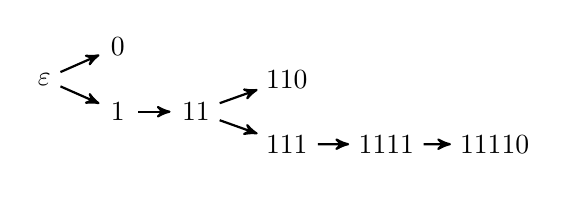
\begin{tikzpicture}[->,>=stealth',auto,thick, scale = 0.55,state/.style={circle,inner sep=2pt}]
	\node [state] at (-0.2,0) (r) {$\varepsilon$};
	\node [state] at (1.5,0.75) (n0) {$0$};
	\node [state] at (1.5,-0.75) (n1) {$1$};
	\node [state] at (3.3,-0.75) (n11) {$11$};
	\node [state] at (5.4,0) (n110) {$110$};
	\node [state] at (5.4,-1.5) (n111) {$111$};
	\node [state] at (7.7,-1.5) (n1111) {$1111$};
	\node [state] at (10.2,-1.5) (n11110) {$11110$};
	
	\path[->]
	(r) edge (n1)
	(r) edge (n0)
	(n1) edge (n11)
	(n11) edge (n110)
	(n11) edge (n111)
	(n111) edge (n1111)
	(n1111) edge (n11110);  	
\end{tikzpicture} 
\end{center}
In this case, we have that $q = \{\varepsilon, 0, 1, 11, 110, 111, 1111, 11110\}$, so $q$ is a finite and prefix-closed subset of $\bB = \{0,1\}^*$. The owner of each block $b \in q \smallsetminus \{ \varepsilon\}$ is given by the  the last symbol of $b$; for instance, we have that $\owner(11) = 1$ and $\owner(11110) = 0$. Moreover, the longest path in $q$ is $\pi = \{\varepsilon, 1, 11, 111, 1111, 11110\}$, so that the blockchain of $q$ is $\pi$ (in symbols, $\bchain(q) = \pi$). 
%Thus, we have that the blocks that belong to the blockchain of $q$ are $\varepsilon$, $1$, $11$, $111$, $1111$, $11110$, since these are precisely the blocks in $q$ in the path from $\varepsilon$ to $11110$ (in symbols, $\epath(\bchain(q)) = \{\varepsilon, 1, 11, 111, 1111, 11110\}$). Notice that the information about these blocks is important as the reward of each player depends on the blocks that belong to her in the blockchain. For instance, if the reward for each block is a constant $c$, then we have that the reward of player 1 is $4 c$ in $q$, as four blocks in the blockchain of $q$ belong to this player. 
Finally, notice that $|q| = 8$, as $q$ is a set consisting of eight blocks.

	Assume now that $q'$ is the following state of the game:
	\begin{center}
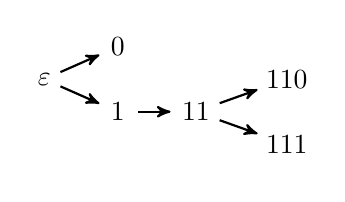
\begin{tikzpicture}[->,>=stealth',auto,thick, scale = 0.55,state/.style={circle,inner sep=2pt}]
	\node [state] at (-0.2,0) (r) {$\varepsilon$};
	\node [state] at (1.5,0.75) (n0) {$0$};
	\node [state] at (1.5,-0.75) (n1) {$1$};
	\node [state] at (3.3,-0.75) (n11) {$11$};
	\node [state] at (5.4,0) (n110) {$110$};
	\node [state] at (5.4,-1.5) (n111) {$111$};

	\path[->]
	(r) edge (n1)
	(r) edge (n0)
	(n1) edge (n11)
	(n11) edge (n110)
	(n11) edge (n111);
\end{tikzpicture} 
\end{center}
In this case, we have that $\bchain(q')$ is not defined since the paths $\pi_1 = \{\varepsilon, 1, 11, 110\}$ and $\pi_2 = \{\varepsilon, 1, 11, 111\}$ are tied for the longest path in $q'$. \qed
\end{example}


Real-life bitcoin blocks also contain transactions that indicate movement of money in the system, and thus there are 
several different blocks that a player $p$ can use to extend the current state when mining upon a block $b$ (e.g, depending  on the ordering of transactions, or the nonce being used to announce the block). Since we are interested primarily in miners behaviour, we just focus on the owner of the block following $b$, and do not consider the possibility of two different blocks belonging to $p$ being added on top of $b$. Alternatively, if we consider the Bitcoin protocol, we could say that all the different blocks that $p$ can put on top of $b$ are considered as~equivalent. 
%\juan{moving this to the reward section}
%\etienne{We may have to specify that it is under the assumption that there are no fees or that they are negligible.} \marcelo{Etienne is right about this, depending on the transactions included in the block the reward could be different. I don't think we should talk about reward here.}

\subsection{Actions of a miner}
On each step, miners looking to maximize their rewards choose a block in the current state, and attempt to mine on top of this block. Thus, in each turn, each of the players race to place the next block in the state, and only one of them succeeds. The probability of succeeding is directly related to the comparative amount of hash power available to this player, the more hash power the likely it is that she will mine the next block before the rest of the players. Once a player places a block, this block is added to the current state, obtaining a different state from which the game continues.

Let $p \in \bP$. Given a block $b \in \bB$ and a state $q \in \bQ$, we denote by $\mine(p,b,q)$ an action played in the mining game in which player $p$ mines on top of block $b$. Such an action $\mine(p,b,q)$ is considered to be valid if $b \in q$ and $b\cdot p \not\in q$. The set of valid actions for player $p$ is collected in the set:
\begin{multline*}
\bA_p \ = \ \{ \mine(p,b,q) \mid b \in \bB, q \in \bQ \text{ and}\\\mine(p,b,q) \text{ is a valid action}\}.
\end{multline*}
Moreover, given $a \in \bA_p$ with $a = \mine(p,b,q)$, the result of applying $a$ to $q$, denoted by $a(q)$, is defined as the state $q \cup \{b \cdot p\}$. Finally, we denote by $\bA$ the set of combined actions for the $m$ players, that is, $\bA = \bA_0 \times \bA_1 \times \cdots \times \bA_{m-1}$.

\subsection{The pay-off of a miner}
The Bitcoin protocol give reward to the owner of a block if it is part of the blockchain and has been confirmed by 100 blocks. A payment function which closely follows this protocol has been introduced in \cite{}, however it adds the constraint that for every level of the state's tree only one block give a reward (the first one which has been confirmed by 100 blocks). Due to this constraint if a fork longer than 100 blocks would happen, some blocks belonging to the new blockchain won't give any reward to their owners (which contradicts the bitcoin's rules). As a matter of fact the model nullify the incentive of performing a fork longer than 100 \cite{}. One could argue that a fork longer than 100 would destroy the market confidence and therefore can be ignored. It might be the case with the current state of crypto-currencies, but as the technology become more widely adopted (government or bank), such argument can not be use any-more.

In stochastic game, the pay-off of a player $p \in \bP$, is given by a function $r_p: \bQ \times \bA \mapsto \mathbb{R}$, and the payoff function of the game is $\bR = (r_0, r_1, \ldots, r_{m-1})$.
As the pay-off of a player is determined by the state and not the history of states, a function which rewards players once and only once for each block they own in the blockchain, can not be build (see example \ref{eximpo}). We propose a model where on every states, we pay miners a constant $c$ for each of the blocks they already have in the blockchain, plus the new block they will potentially mine. This model puts a strong incentive in maintaining blocks in the blockchain and does not nullify the incentive to fork.
The main concern regarding this pay-off model, is that we might end-up giving reward to player multiple times for the same block (once for each state where the block belongs to the blockchain). In the following sections we address this specific matter \ref{} and formally defines our pay-off functions \ref{}. 

Note that if in the general case a pay-off is a function from $\bQ \times \bA$ to $\mathbb{R}$, in our model the pay-off for a player $p$ does not depend on the action of other players. Hence we can extend the definition such that for any state $q$ and any player $p$ we have $r_p(q) = r_p(q',(\ba,a_p))$ with $q' = q \setminus b$ a state and $a_p = mine(p,b,q')$ a valid action.  
 
 
\subsection{The definition of the game}
As a last component of the game, we assume that $\pr : \bQ \times \bA \times \bQ \to [0,1]$ is a transition probability function satisfying that for every state $q \in \bQ$ and combined action $\ba = (a_0, a_1, \ldots, a_{m-1})$ in $\bA$:
\begin{eqnarray*}\label{eq-prop}
\sum_{p=0}^{m-1} \pr(q, \ba, a_p(q)) & = & 1.
\end{eqnarray*}
Notice that if $p_1$ and $p_2$ are two different players, then for every action $a_1 \in \bA_{p_1}$, every action $a_2 \in \bA_{p_2}$ and every state $q \in \bQ$, it holds that $a_1(q) \neq a_2(q)$. Thus, we can think of $\pr(q, \ba, a_p(q))$ as the probability that player $p$ places the next block, which will generate the state $a_p(q)$. 

Summing up, from now on we consider an infinite stochastic game $\Gamma = (\bP,\bA,\bQ,\bR,\pr)$, where $\bP$ is the set of players, $\bA$ is the set of combined actions, $\bQ$ is the set of states, $\bR$ is the pay-off function and $\pr$ is the transition probability function.
%\begin{itemize}
%	\item $\bP$ is the set of players.
%	\item $\bA$ is the set of possible actions.
%	\item $\bQ$ is the set of states.
%	\item $\bR$ is the pay-off function.
%	\item $\pr$ is the transition probability function.
%\end{itemize} 

\subsubsection{Games with constant hash power}
%\label{sec-simp}
Recall that the probability that action $a_p$ is indeed executed is given by $\pr(q, \ba, a_p(q))$. As we have mentioned, such a probability is directly related with the hash power of player $p$, the more hash power the likely it is that action $a_p$ is executed and $p$ mines the next block before the rest of the players. In what follows, we assume that the hash power of each player does not change during the mining game, which is captured by the following condition:
\begin{itemize}
\item For every $q, q' \in \bQ$, every $\ba, \ba' \in \bA$ such that $\ba = (a_0, a_1$, $\ldots$, $a_{m-1})$ and $\ba' = (a'_0, a'_1, \ldots, a'_{m-1})$,  and every player $p \in \bP$, it holds that $\pr(q, \ba, a_p(q)) = \pr(q', \ba', a'_p(q'))$.
\end{itemize}
Thus, we assume from now on that this condition is satisfied. In particular, for each player $p \in \bP$, we assume that that 
$\pr(q, \ba, a_p(q)) = h_p$ for every $q \in \bQ$ and $\ba \in \bA$ with $\ba = (a_0, a_1, \ldots, a_{m-1})$, and we refer to $h_p$ as the hash power of player $p$. 
%Moreover, we define $\bH = (h_0, h_1, \ldots, h_{m-1})$ as the hash power distribution, and we replace $\pr$ by $\bH$ in the definition of an an infinite stochastic game, so that $\Gamma = (\bP,\bA,\bQ,\bR,\bH)$. 
Moreover, we assume that $h_p > 0$ for every player $p \in \bP$, as if this not the case then $p$ can just be removed from the mining game. 

\subsection{Utility and equilibria of the game}
We have defined a game that can capture miners' interactions. A fundamental component of such a game is the strategy that each player decides to take, which combined determine the utility of each player. In particular, miners take actions and decide about strategies trying to maximize their utility. In this sense, a stationary equilibrium of the game is a fundamental piece of information about miners' behavior, as such an equilibrium is a combination of players' strategies where no miner has an incentive to perform a different action. The notions of strategy, utility and stationary equilibrium are the last components of our game-theoretical characterization of mining in Bitcoin, and they are defined in this section.

A strategy for a player $p \in \bP$ is a function $s : \bQ \rightarrow \bA_p$. 
We define $\bS_p$ as the set of all strategies for player $p$, and $\bS = \bS_0 \times \bS_{1} \times \cdots \times \bS_{m-1}$ as the set of combined strategies for the game (recall that we are assuming that $\bP = \{0, 1, \ldots, m-1\}$ is the set of players). 

As usual, we are interested in understanding which strategies fare better than others, which we capture by the notions of  utility and equilibrium. To define these, we need some additional notation. 
Let $\bs = (s_0, s_1, \ldots, s_{m-1})$ be a strategy in $\bS$. Then given $q \in \bQ$, define $\bs(q)$ as the combined action $(s_0(q), s_1(q), \ldots, s_{m-1}(q))$. Moreover, given an initial state $q_0 \in \bQ$, 
the probability of reaching state $q \in \bQ$, denoted by $\pr^{\bs}(q \mid q_0)$, is defined as 0 if $q_0 \not\subseteq q$, and otherwise it is recursively defined as follows: if $q =  q_0$, then $\pr^{\bs}(q \mid q_0) = 1$; otherwise, we have that $|q| - |q_0| = k$, with $k \geq 1$, and
$$
\pr^{\bs}(q \mid q_0) =
\sum_{\substack{q' \in \bQ \,:\\ q_0 \subseteq q' \text{ and } |q'| - |q_0| = k-1}}
 \pr^{\bs}(q' \mid q_0) \cdot \pr(q', \bs(q'), q).
 $$
In this definition, if for a player $p$ we have that $s_p(q') = a$ and $a(q') = q$, then $\pr(q', \bs(q'), q) = h_p$. Otherwise, we have that $\pr(q', \bs(q'), q) = 0$. 
%Hence, consistently with the simplification described before, we can replace the transition probability function $\pr$ by the hash power distribution $\bH$ when computing $\pr^{\bs}(q \mid q_0)$. 
It should be noticed that the framework just described corresponds to a Markov chain; in particular, the probability of reaching a state from an initial state is defined in the standard way for Markov chains~\cite{MU05}. However, we are not interested in the steady distribution for such a Markov chain and, thus, we do not explore more this connection in this paper.

We finally have all the necessary ingredients to define the utility of a player in a mining game given a particular strategy. As is common 
when looking at personal utilities, we define it as the summation of the expected rewards, and choose 
to impose a discount for future rewards using a factor $\beta \in (0,1)$. 

\begin{mydef}
\label{def-utility}
The $\beta$--discounted utility of player $p$ for the strategy $\bs$ from the state $q_0$ in 
the mining game, denoted by $u_p(\bs \mid q_0)$, is defined as:
\begin{eqnarray*}
u_p(\bs \mid q_0) & = & (1 - \beta) \cdot  \sum_{q \in \bQ \,:\, q_0 \subseteq q} \beta^{|q|-|q_0|} \cdot  r_p(q) \cdot \pr^{\bs}(q \mid q_0).
\end{eqnarray*}
\end{mydef}
Notice that the value $u_p(\bs \mid q_0)$ may not be defined if the series $\sum_{q \in \bQ \,:\, q_0 \subseteq q} \beta^{|q|-|q_0|} \cdot  r_p(q) \cdot \pr^{\bs}(q \mid q_0)$ diverges. To avoid this problem, from now on we assume that for every pay-off function $\bR = (r_0, \ldots, r_{m-1})$, there exists a polynomial $P$ such that $|r_p(q)| \leq P(|q|)$ for every player $p \in \bP$ and state $q \in \bQ$. Under this simple yet general condition, it is posible to prove that $u_p(\bs \mid q_0)$ is a real number (see Appendix \ref{sec-conver} for a proof of this property). 

As a last ingredient in our formalization, we need to introduce the notion stationary equilibrium.
Given a player $p \in \bP$, a combined strategy $\bs \in \bS$, with $\bs = (s_0,s_1, \ldots, s_{m-1})$, and a strategy $s$ for player $p$ ($s \in \bS_p$), we denote by $(\bs_{-p}, s)$ the strategy $(s_0, s_1, \ldots s_{p-1},s,s_{p+1}, \ldots, s_{m-1})$.
\begin{mydef}
A strategy $\bs$ is a $\beta$--discounted stationary equilibrium from the state $q_0$ in  the %infinite 
mining game if for every player $p \in \bP$ and every strategy $s$ for player $p$ $(s \in\bS_p)$, it holds that:
\begin{eqnarray*}u_p(\bs \mid q_0)  & \geq  & u_p ((\bs_{-p},s) \mid q_0).
\end{eqnarray*}
\end{mydef}
We conclude this section by going deeper into the definition of utility, given the key role it plays in our framework. 
Definition~\ref{def-utility} corresponds to the usual notion of average discounted utility \marcelo{A citation is needed here}. In particular, if the starting point of the game is a state $q_0$, then for every state $q$ such that $q_0 \subseteq q$, the pay-off of a player $p$ in $q$ is $\beta^{|q|-|q_0|} \cdot r_p(q)$, where $|q|-|q_0|$ is the number of steps that have to be performed to reach $q$ from $q_0$ so the discount factor $\beta^{|q|-|q_0|}$ has to be applied. The uncertainty  about reaching state $q$ from $q_0$ is taking into consideration by including the term $\pr^{\bs}(q \mid q_0)$, which tell us that the expected payoff for the state $q$ is $\beta^{|q|-|q_0|} \cdot  r_p(q) \cdot \pr^{\bs}(q \mid q_0)$.  
%
As a last comment on the definition of utility, notice that a block $b$ can be included in an infinite number of states $q$ such that $\pr^{\bs}(q \mid q_0) > 0$. But the reward obtained by a player $p$ for this block $b$ should not be added more than once, which is the reason to include the term $(1 - \beta)$ in the definition of utility. Let us formalize this claim in more precise terms. 

Assume that the reward obtained by a player $p$ for a block $b$ in a state $q$ is given by $r_p(b,q)$, so that $r_p(q) = \sum_{b \in q} r_p(b,q)$. Notice that such decomposition can always be done; in fact, it can be done in a natural and straightforward way for the pay-off functions considered in this paper and in other game-theoretical formalizations of Bitcoin mining \cite{mininggames:2016}. Then we have that:
\begin{align*}
u_p(\bs \mid \{\varepsilon\}) & =  (1 - \beta) \cdot  \sum_{q \in \bQ} \beta^{|q|-|\{\varepsilon\}|} \cdot  r_p(q) \cdot \pr^{\bs}(q \mid \{\varepsilon\})\\
& =  (1 - \beta) \cdot \sum_{q \in \bQ} \beta^{|q|-1} \cdot  \bigg(\sum_{b \in q} r_p(b,q) \bigg) \cdot \pr^{\bs}(q \mid \{\varepsilon\})\\
& = (1 - \beta) \cdot \sum_{b \in \bB} \sum_{q \in \bQ \,:\, b \in q} \beta^{|q|-1} \cdot r_p(b,q) \cdot \pr^{\bs}(q \mid \{\varepsilon\}).
\end{align*}
For the sake of readability, we assume that the game is starting from the initial state $\{\varepsilon\}$ that consists only of the genesis block. Notice that $|\{\varepsilon\}| = 1$, so that the discount factor for a state $q$ is $\beta^{|q|-1}$. Now assume that there is a maximum value for the reward of a block $b$ for player $p$, which is denoted by $M_p(b)$. Thus, we have that there exists $q_1 \in \bQ$ such that $b \in q_1$ and $M_p(b) = r_p(b,q_1)$, and for every $q_2 \in \bQ$ such that $b \in q_2$, it holds that $r_p(b,q_2) \leq M_p(b)$. Again, such an assumption is satisfied by the pay-off functions considered in this paper and in other game-theoretical formalizations of Bitcoin mining \cite{mininggames:2016}. Then we have that:
\begin{align*}
&\sum_{b \in \bB} \sum_{q \in \bQ \,:\, b \in q} \beta^{|q|-1} \cdot r_p(b,q) \cdot \pr^{\bs}(q \mid \{\varepsilon\})
\ \leq \\  
&\hspace{40pt}  \sum_{b \in \bB} \sum_{q \in \bQ \,:\, b \in q} \beta^{|q|-1} \cdot M_p(b) \cdot \pr^{\bs}(q \mid \{\varepsilon\}) \ =\\
&\hspace{40pt}  \sum_{b \in \bB} M_p(b) \cdot\bigg(\sum_{q \in \bQ \,:\, b \in q} \beta^{|q|-1}  \cdot \pr^{\bs}(q \mid \{\varepsilon\})\bigg) \ \leq\\
&\hspace{40pt}  \sum_{b \in \bB} M_p(b) \cdot\bigg(\sum_{q \in \bQ \,:\, |q| \geq |b|+1} \beta^{|q|-1}  \cdot \pr^{\bs}(q \mid \{\varepsilon\})\bigg) \ = \\
&\hspace{40pt}  \sum_{b \in \bB} M_p(b) \cdot\bigg(\sum_{i=|b|+1}^\infty \sum_{q \in \bQ \,:\, |q| = i} \beta^{|q|-1}  \cdot \pr^{\bs}(q \mid \{\varepsilon\})\bigg) \ = \\
&\hspace{40pt}  \sum_{b \in \bB} M_p(b) \cdot\bigg(\sum_{i=|b|+1}^\infty \beta^{i-1} \cdot \sum_{q \in \bQ \,:\, |q| = i} \pr^{\bs}(q \mid \{\varepsilon\})\bigg).
\end{align*}
By the definition of the transition probability function $\pr^{\bs}$, it is straightforward to prove that $\sum_{q \in \bQ \,:\, |q| = i} \pr^{\bs}(q \mid \{\varepsilon\}) = 1$. Hence, we conclude that:
\begin{align*}
&\sum_{b \in \bB} M_p(b) \cdot\bigg(\sum_{i=|b|+1}^\infty \beta^{i-1} \cdot \sum_{q \in \bQ \,:\, |q| = i} \pr^{\bs}(q \mid \{\varepsilon\})\bigg) \ = \\
&\hspace{60pt}  \sum_{b \in \bB} M_p(b) \cdot\bigg(\sum_{i=|b|+1}^\infty \beta^{i-1}\bigg) \ = \\
&\hspace{60pt}  \sum_{b \in \bB} M_p(b) \cdot \beta^{|b|} \cdot \bigg(\sum_{j=0}^\infty \beta^{j}\bigg) \ = \\
&\hspace{60pt}  \sum_{b \in \bB} M_p(b) \cdot \beta^{|b|} \cdot \frac{1}{1-\beta},
\end{align*}
where $|b|$ is the length of block $b$ considered as a string. Therefore, we finally conclude that:
\begin{eqnarray*}
u_p(\bs \mid \{\varepsilon\}) & \leq &  \sum_{b \in \bB} \beta^{|b|} \cdot M_p(b).
\end{eqnarray*}
Thus, the pay-off obtained by player $p$ for a block $b$ is at most $\beta^{|b|} \cdot M_p(b)$, that is, the maximum reward that she can obtained for the block $b$ in a state multiplied by the discount factor $\beta^{|b|}$, where $|b|$ is the minimum number of steps that have to be performed to reach a state containing $b$ from the initial state $\{\varepsilon\}$.

\marcelo{The justification of the utility function is long, we can move the proof to the appendix and only keep the bound $u_p(\bs \mid \{\varepsilon\}) \leq \sum_{b \in \bB} \beta^{|b|} \cdot M_p(b)$.}

%Along the paper we will also consider games ending in a finite number of steps. For these games we redefine the notion of $\beta$-discounted utilities by summing up the rewards only up to $n$, and define the notion of a $\beta$-discounted equilibrium accordingly. 
%\marcelo{We are not going to consider games ending in a finite number of steps in this paper, right?}

%\marcelo{In these definitions we are assuming that $u_p(\bs \mid q_0)$ is defined, which could not be the case if the series diverges. We should say something about this.}
%\francisco{True. Something like ``$r$ is a decreasing function and card$(Q)$ is controlled by $p^{|q|}$'' (worst case scenario, every player forks), so we should be OK.}

\iffalse

\subsection{Pay-off of a miner (extended version)}


\etienne{I still have to work on the actual wording, but i think it will look like that. I choosed to push the graph in appendix for space reasons, what do u think ?}

In stochastic game,the pay-off of a player $p \in \bP$, is given by a function $r_p: \bQ \times \bA \mapsto \mathbb{R}$, and the payoff function of the game is $\bR = (r_0, r_1, \ldots, r_{m-1})$.
But how should the function $r_p(q,\ba)$ look like? Recall that one of the rules of bitcoin is that the money can only 
be spent when it is given in blocks that are part of the blockchain. Thus, the first idea that comes into mind is to 
reward players every time they put a block in the blockchain. However, this is not a good function, as it is not possible to build a pay-off function which rewards them once and only once for each block in the blockchain (see example \ref{eximpo}).

\begin{myex} 
\label{eximpo}
\begin{figure}
\begin{center}
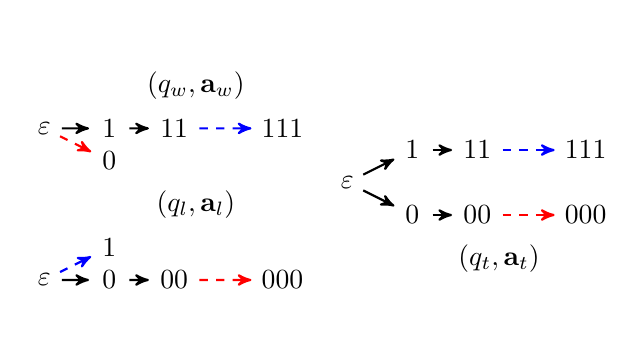
\begin{tikzpicture}[->,>=stealth',auto,thick, scale = 0.55,state/.style={circle,inner sep=2pt}]

    % The graph A
    \node [state] at (3.5,2.25) (name1) {$(q_w,\ba_w)$};
	\node [state] at (0,1.25) (Ra0) {$\varepsilon$};
	\node [state] at (1.5,0.5) (0a0) {$0$};
	\node [state] at (1.5,1.25) (1a0) {$1$};
	\node [state] at (3,1.25) (11a0) {$11$};
	\node [state] at (5.5,1.25) (111a0) {$111$};
	
	 % The graph A
	\node [state] at (0,-2.25) (Ra1) {$\varepsilon$};
	\node [state] at (1.5,-1.5) (0a1) {$1$};
	\node [state] at (1.5,-2.25) (1a1) {$0$};
	\node [state] at (3,-2.25) (11a1) {$00$};
	\node [state] at (5.5,-2.25) (111a1) {$000$};
	\node [state] at (3.5,-0.5) (name2) {$(q_l,\ba_l)$};
	
	% The graph A
	\node [state] at (7,0) (Ra) {$\varepsilon$};
	\node [state] at (8.5,0.75) (1a) {$1$};
	\node [state] at (8.5,-0.75) (0a) {$0$};
	\node [state] at (10,0.75) (11a) {$11$};
	\node [state] at (10,-0.75) (00a) {$00$};
	\node [state] at (12.5,0.75) (111a) {$111$};
	\node [state] at (12.5,-0.75) (000a) {$000$};
	\node [state] at (10.5,-1.75) (name3) {$(q_t,\ba_t)$};	
	
	% Graph edges
	\path[->]
	(Ra) edge (1a)
	(Ra) edge (0a)
	(1a) edge (11a)
	(0a) edge (00a)
	(Ra1) edge (1a1)
	(1a1) edge (11a1)
	(Ra0) edge (1a0)
	(1a0) edge (11a0)
	;  	
	
	% Graph edges
	\path[dashed,blue]
	(Ra1) edge (0a1)
	(11a) edge (111a)
	(11a0) edge (111a0)
	;  	
	
	\path[dashed,red]
	(Ra0) edge (0a0)
	(00a) edge (000a)
	(11a1) edge (111a1)
	;


\end{tikzpicture} 
\end{center}
\caption{An example showing that I should want to try to compete when some other player forks on my blocks. \label{fig-impo}}
\end{figure}



Consider a pay-off function $r_1$ for player $1$, it is immediate to understand that in the situation described by $q_l$ the value $r_1(q_l,\ba_l)$ should be $0$, indeed player $1$ did not put any new block in the blockchain. While in the situation described in $q_w$, $r_1(q_w,\ba_w)$ should reward the player $1$ for his block $111$.
\\Now consider the tie situation described in $q_t$. What should be the value of $r_1(q_t,\ba_t)$? Either $r_1(q_t,\ba_t)$ only rewards player 1 for his block $111$, and if $q_t$ has been reach through $q_l$ then he would never has been paid for the block $1$. Or $r_1(q_t,\ba_t)$ rewards player 1 for every blocks involved in the tie and if $q_t$ is reach trough $q_w$, he would have been paid twice for the blocks $1$ and $11$. The pay-off not relying on the history of states, cannot distinguish those two situations hence it is not possible to build a pay-off function which pay once and only once the player for each block in the blockchain.

\end{myex} 

Ideally, one would like to reward players according to the blocks they have in the blockchain when the game terminates (or the limit of that number, in the case of infinite games). The problem is that we cannot really know what this pay-off will be until the game is actually finished, and thus we cannot model this pay-off in our stochastic game setting. 
What we do instead is to use a heuristic for this reward called cumulative pay-off model and denoted $r_p^c(.)$. On each turn, we pay miners a constant $c$ for each of the blocks they already have in the blockchain, plus the new block they have potentially mining them. This clearly puts a strong incentive in maintaining blocks, but also on mining new blocks on the blockchain. 
\\Note that in the general case a pay-off is a function from $\bQ \times \bA$ to $\mathbb{R}$, in our model the pay-off of player $p$ does not depend on the action of other players. Hence we extend the definition of the cumulative pay-off function such that for any state $q$ and any player $p$ we have $r_p^c(q) = r_p^c(q',(\ba,a_p))$ with $q' = q \setminus b$ and $a_p = mine(p,b,q')$. We also consider a function where the reward for each new block in the blockchain decreases by a constant factor $\alpha$. We will formally define our cumulative payoff functions in the following sections. 


The main concern regarding this pay-off function called cumulative pay-off, is that the early blocks may have a lot more value than the later ones (not because of a decreasing reward, but because early blocks are counted multiple times).
In order to show that this problem is not as strong as it might seems, we compared the sum of the rewards obtained under the cumulative, relative \cite{} and absolute \cite{} pay-off models on pseudo-randomly generated  blockchains. We considere a fix number of blocks distrubuted upon players $\bP$ and we assume they always mined upon the blockchain (default behaviour). Therefore the only variable between two iterations is the position of the blocks own by each players. The total number of blocks at the end of each iteration is 100.000 and we have done 1000 iterations. Let $i \in \{1\cdots 1000\}$, we denote by $q_i$ the final state of the iteration. For any state $q \subseteq q_i$ and any player $p \in \bP$ we denote $r_p^a(q)$ resp. $r_p^r(q)$ the absolute resp. relative pay-off function. We have that $r_p^a(q) = c$ if $owner(bc(q)) = p$ and $r_p^a(q) = 0$ otherwise. And that $r_p^r(q) = \frac{c}{|q|}$ if $owner(bc(q)) = p$ and $r_p^r(q) = 0$ otherwise. Finally with $$R_p^x(q_i) = \frac{\sum\limits_{q \subseteq q_i} r_p^x(q)}{\sum\limits_{p' \in \bP}\sum\limits_{q \subseteq q_i} r_{p'}^x(q)} $$ we call maximum difference the value:\\ $\underset{p \in \bP}{max}\left(\underset{{i \in \{1 \cdots 10
00\}}}{max}(R_p^x(q_i)) - \underset{{i \in \{1 \cdots 10
00\}}}{min}(R_p^x(q_i))\right)$\\and average difference the value: $\underset{{i,i' \in \{1 \cdots 10
00\}}}{average}(|R_p^x(q_i) - R_p^x(q_{i'})|) $.

\begin{figure}
\begin{tabular}{c|c|c|}
. & maxium difference & average difference   \\
\hline
constant pay-off & 0 & 0 \\
\hline
relative pay-off & x.x &  x.x \\
\hline
cumulative pay-off &  x.x &  x.x \\
\end{tabular}
\caption{Results of the simulation for absolute, relative and cumulative models}
\end{figure}

As you can see in the table \ref{}, the cumulative model yields to a behaviour inbetween the constant and relative models. Therefore, even if the value for the early blocks of the blockchain is higher than the value for the later ones, the difference between them is reasonable. More details and results about this experimentation are available in appendix \ref{}.

An other possible pay-off function presented in \cite{}, introduced a delay $d$ before rewarding a player for a block. Moreover this pay-off also insure that only one block for each depth is going to receive a payment (the first one for which the delay $d$ is achieve). It is really close to the bitcoin protocol as miners have to wait 100 blocks in order to use their coin-base transaction bitcoins, however the constraint that only one block per depth can be paid nullify the incentive of performing a fork longer than $d$. One could argue that a fork longer than $d$ would destroy the market confidence hence the value and therefore can be ignored. It might be the case with the current state of crypto-currencies, but if the technology become more widely adopted (government or bank), such argument can not be use any-more.



%The other issue is what to do when the blockchain is contested, and there are at least two paths sharing the maximal length. A simple solution 
%would be to declare that players receive no pay-off when this happens. But again, this would lead to strange behaviours in which players with several blocks buried deep in the blockchain would receive no reward for this blocks because of a contest in the newer parts of the blockchain. 
%In order to avoid this scenario, we choose to maintain the reward for blocks buried deep in the blockchain even when there is a contest, 
%and formalise this as follows. 
\fi

\iffalse

\begin{myex} 
\label{eximpo}
\begin{figure}
\begin{center}
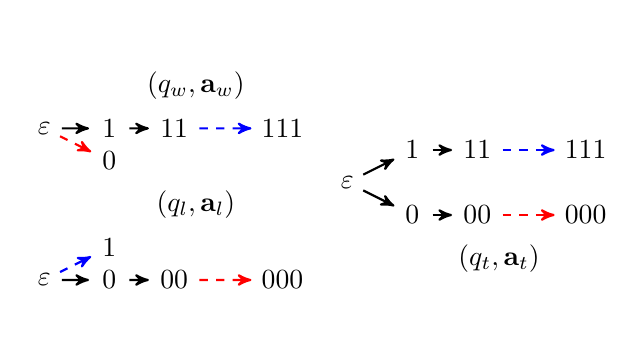
\begin{tikzpicture}[->,>=stealth',auto,thick, scale = 0.55,state/.style={circle,inner sep=2pt}]

    % The graph A
    \node [state] at (3.5,2.25) (name1) {$(q_w,\ba_w)$};
	\node [state] at (0,1.25) (Ra0) {$\varepsilon$};
	\node [state] at (1.5,0.5) (0a0) {$0$};
	\node [state] at (1.5,1.25) (1a0) {$1$};
	\node [state] at (3,1.25) (11a0) {$11$};
	\node [state] at (5.5,1.25) (111a0) {$111$};
	
	 % The graph A
	\node [state] at (0,-2.25) (Ra1) {$\varepsilon$};
	\node [state] at (1.5,-1.5) (0a1) {$1$};
	\node [state] at (1.5,-2.25) (1a1) {$0$};
	\node [state] at (3,-2.25) (11a1) {$00$};
	\node [state] at (5.5,-2.25) (111a1) {$000$};
	\node [state] at (3.5,-0.5) (name2) {$(q_l,\ba_l)$};
	
	% The graph A
	\node [state] at (7,0) (Ra) {$\varepsilon$};
	\node [state] at (8.5,0.75) (1a) {$1$};
	\node [state] at (8.5,-0.75) (0a) {$0$};
	\node [state] at (10,0.75) (11a) {$11$};
	\node [state] at (10,-0.75) (00a) {$00$};
	\node [state] at (12.5,0.75) (111a) {$111$};
	\node [state] at (12.5,-0.75) (000a) {$000$};
	\node [state] at (10.5,-1.75) (name3) {$(q_t,\ba_t)$};	
	
	% Graph edges
	\path[->]
	(Ra) edge (1a)
	(Ra) edge (0a)
	(1a) edge (11a)
	(0a) edge (00a)
	(Ra1) edge (1a1)
	(1a1) edge (11a1)
	(Ra0) edge (1a0)
	(1a0) edge (11a0)
	;  	
	
	% Graph edges
	\path[dashed,blue]
	(Ra1) edge (0a1)
	(11a) edge (111a)
	(11a0) edge (111a0)
	;  	
	
	\path[dashed,red]
	(Ra0) edge (0a0)
	(00a) edge (000a)
	(11a1) edge (111a1)
	;


\end{tikzpicture} 
\end{center}
\caption{An example showing that I should want to try to compete when some other player forks on my blocks. \label{fig-impo}}
\end{figure}

Consider a pay-off function $r_1$ for player $1$, it is immediate to understand that in the situation described by $q_l$ the value $r_1(q_l,\ba_l)$ should be $0$, indeed player $1$ did not put any new block in the blockchain. While in the situation described in $q_w$, $r_1(q_w,\ba_w)$ should reward the player $1$ for his block $111$.
\\Now consider the tie situation described in $q_t$. What should be the value of $r_1(q_t,\ba_t)$? Either $r_1(q_t,\ba_t)$ only rewards player 1 for his block $111$, and if $q_t$ has been reach through $q_l$ then he would never has been paid for the block $1$. Or $r_1(q_t,\ba_t)$ rewards player 1 for every blocks involved in the tie and if $q_t$ is reach trough $q_w$, he would have been paid twice for the blocks $1$ and $11$. The pay-off not relying on the history of states, cannot distinguish those two situations hence it is not possible to build a pay-off function which pay once and only once the player for each block in the blockchain.

\end{myex} 
\fi




	%!TEX root = main.tex


\section{Equilibria in games with constant payoff}
\label{sec-const_rew}

The first version of the game we analyse is when the payoff function $r_p(q)$ pays each block in the blockchain the same amount $c$. While this does not reflect the reality of the Bitcoin protocol, this simplification serves as a good baseline for future results, and it establishes the main techniques we will use. Furthermore, the results we obtain here could serve as a good recommendation of how the Bitcoin protocol can be modified in order to enforce fair behaviour of the miners when the block reward becomes insignificant.
\marcelo{We need to change this considering the more general view of our framework for cryptocurrencies.}

\subsection{Defining constant pay-off}
When considering the constant reward $c$ for each block, $r_p(q)$ will equal $c$ times the number of blocks owned by $p$ in the blockchain $\bchain(q)$ of $q$, when the latter is defined. On the other hand, when $\bchain(q)$ is not defined it might seem tempting to simply define $r_p(q) = 0$. However, even if there is more than one longest path from the root of $q$ to its leaves, it might be the case that all such paths share a common subpath. In fact, this often happens in the Bitcoin's network, when two blocks were mined on top of the same block (with a small time delay). While in this situation the blockchain is not defined, the miners know that they will at least be able to collect their reward on the portion of the state these two paths agree on. Figure \ref{fig-simple-fork} illustrates this situation. 

\begin{figure}
\begin{center}
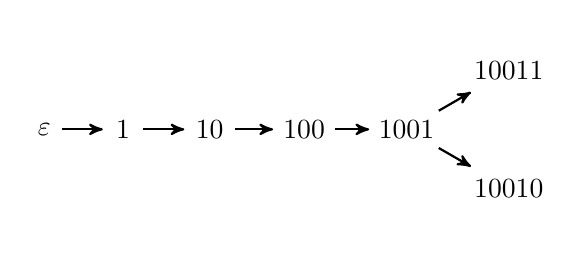
\begin{tikzpicture}[->,>=stealth',auto,thick, scale = 1.0,state/.style={circle,inner sep=2pt}]

    % The graph
	\node [state] at (0,0) (R) {$\varepsilon$};
	\node [state] at (1,0) (1) {$1$};
	\node [state] at (2.1,0) (10) {$10$};
	\node [state] at (3.3,0) (100) {$100$};
	\node [state] at (4.6,0) (1001) {$1001$};
	\node [state] at (5.9,0.75) (10011) {$10011$};
	\node [state] at (5.9,-0.75) (10010) {$10010$};	
	
	% Graph edges
	\path[->]
	(R) edge (1)
	(1) edge (10)
	(10) edge (100)
	(100) edge (1001)
	(1001) edge (10011)
	(1001) edge (10010)
	;  	
	


\end{tikzpicture} 
\end{center}
\caption{Although two paths are competing to become a blockchain, the blocks up to 1001 will contribute to the reward in each case. \label{fig-simple-fork}}
\end{figure}

In order to model the aforementioned scenario we need to introduce some notation.
Recall that a block $b$ is a string over the alphabet $\bP$, and we use notation $|b|$ for the length of $b$ as a string. Moreover, given blocks $b_1, b_2$, we use notation $b_1 \preceq b_2$ to indicate that $b_1$ is a prefix of $b_2$  when considered as strings. Then we define: 
\begin{eqnarray*}
\longest(q) & = & \{ b \in q \mid \text{for every } b' \in q: |b'| \leq |b|\}\\
\meet(q) & = & \{b \in q \mid \text{for every } b' \in \longest(q): b \preceq b'\}.
\end{eqnarray*}
Intuitively, $\longest(q)$ contains the leaves of all paths in the state $q$ that are currently competing for the blockchain, and $\meet(q)$ is the path from the genesis block to the last block for which all these paths agree on. For instance, if $q$ is the state from Figure~\ref{fig-simple-fork}, then we have that $\longest(q)=\{10011,10010\}$, and $\meet(q)=\{\varepsilon, 1, 10, 100, 1001\}$. Notice that $\meet(q)$ is well defined as $\preceq$ is a linear order on the finite and non-empty set $\{b \in q \mid \text{for every } b' \in \longest(q): b \preceq b'\}$. Also notice that $\meet(q)=\bchain(q)$, whenever $\bchain(q)$ is defined.


As mentioned before, the pay-off function will reward a player for the blocks in $\meet(q)$. Thus, to define the pay-off, we need to identify who is the owner of each one of these blocks, which is done by considering the function $\chi_p$, for each $p \in \bP$. More precisely, given $b \in \bB$, we have that:
\begin{eqnarray*}
\chi_p(b) & = & 
\begin{cases}
1 & \text{if } \owner(b) = p\\
0 & \text{otherwise}
\end{cases}
\end{eqnarray*}
We can finally define the payoff function we consider in this section, which we call \textbf{constant reward}. For a player $p$, we define it as 
\begin{eqnarray*}
r_p(q) & = & 
{\displaystyle c \cdot \sum_{b \in \meet(q)} \chi_p(b),}
\end{eqnarray*}
\martin{this reads odd since we do not use meet here. Is it correct?} \marcelo{I don't understand this comment, meet is used in the expression above.}
where $c$ is a positive real number. As mentioned above, this function is well defined since $\meet(q)$ always exists. Moreover, if $q$ has a blockchain, then we have that $\meet(q) = \bchain(q)$ and, hence, the pay-off function is defined for the blockchain of $q$.
% when the latter is defined for the state $q$.
%Here we use notation $b[i]$ for the $i$-th symbol in $b$, where $i \in \{1, \ldots, |b|\}$. 
% and $d \in \mathbb{N}$. Here the number $d$ is the amount of confirmations needed to spend the block (6 in the case of Bitcoin).
 
 \subsection{The default strategy maximizes the utility}

Let us start with analysing the most obvious strategy for all players: regardless of what everyone else does, keep mining on the blockchain, which is called the \emph{default} strategy.
More precisely, a player following the default strategy tries to mine upon the final block that appears in the blockchain of a state $q$. If the blockchain in $q$ does not exist, meaning that there are al least two longest paths from the genesis block, then the player tries to mine on the final block of one of these paths according to her rewards in them; she chooses the one that maximizes her reward, which in the case of constant reward means the path that contains the largest number of blocks belonging to her (if there is more than one of these paths, then between the final blocks of these paths she chooses the first according to a lexicographic order on the strings in $\{0, \ldots, m-1\}^*$). 
Notice that this is called the default strategy as it reflects the desired behaviour of the miners participating in the Bitcoin network.  For a player $p$, let us denote this strategy 
by $\df_p$, and consider the combined strategy $\cdf = (\df_0,\df_1,\dots,\df_{m-1})$. 
%Notice that under this strategy, each state $q$ consists of a single path from the genesis block $\varepsilon$ to the final block in $\bchain(q)$.

We can now easily calculate the utility of player $p$ under $\cdf$. Intuitively, a player $p$ will receive a fraction $h_p$ of the next block that is being placed in the blockchain, corresponding to her hash power. Therefore, at stage $i$ of the mining game, $i$ blocks will be placed in the blockchain defined by the game, and the expected amount of blocks owned by the player $p$ will be $h_p\cdot i$. This means that the total utility for player $p$ amounts to 
$$u_p(\cdf \mid \varepsilon) \ \ = \ \ (1 - \beta) \cdot h_p \cdot c\cdot \sum_{i=0}^{\infty}i \cdot \beta^{i} \ \ =  \ \ h_p\cdot c \cdot \frac{\beta}{(1-\beta)}.$$

%% Juan: I think it is way too nahive to put the analytical form of this
%$$u_p(\bs \mid q_0) = c\cdot h_p \cdot \sum_{i=0}^{\infty}i \cdot \beta^{i} \text{,}\ \ \ \ \text{ which evaluates to }\frac{c\cdot h_p}{(1-\beta)^2}.$$ %(recall that $q_0$ is the genesis block). 

The question then is: can any player do better? As we show in the following theorem, the answer is no as the default strategy maximizes the utility. 
\begin{mythm}\label{thm-conts_dom_str}
Let $p$ be a player, $\beta$ be a discount factor in $(0,1)$ and $u_p$ be the utility function defined in terms of $\beta$. Then for every combined strategy $\bs$:
\begin{eqnarray*}
u_p(\bs \mid \varepsilon) & \leq & u_p(\cdf \mid \varepsilon)
\end{eqnarray*}
\end{mythm} 

\begin{proof}
Let $\bs= (s_0, \ldots, s_{m-1})$ be an arbitrary combined strategy, and define $Q_\bs = \{q \in \bQ \mid \pr^\bs(q \mid \varepsilon) > 0\}$. Thus, $Q_\bs$ is the set of all states that can be reached from the genesis block using the combined strategy $\bs$. For example, we have that $Q_\cdf$ is the set of states $q$ such that $q$ consists of a single path from the genesis block to the final block in $\bchain(q)$.
Moreover, define a mapping $\sigma: Q_{\bs} \rightarrow 2^{Q_\cdf}$ as follows. Given two states $q_1, q_2$, we say that $q_2$ can be reached from $q_1$ in one step if $q_2 = q_1 \cup \{ b \cdot p' \}$, where $b \in \bB$, $p' \in \bP$ and $b \cdot p' \not\in q_1$ (recall that $\bB = \{0, \ldots, m-1\}^*$ and $\bP = \{0, \ldots, m-1\}$); that is, we have that $q_2$ can be reached from $q_1$ in one step  if $q_2$ is the result of applying action $\mine(p', b, q_1)$, where $\mine(p', b, q_1)$ is a valid action for player $p'$. 
Then for each state $q \in Q_{\bs}$, consider all distinct sequences $\rho = q_0,\dots,q_n$ such that $q_{i+1}$ can be reached from 
$q_i$ in one step ($i \in \{1, \ldots, n-1\}$), $q_0 = \varepsilon$ and $q_n = q$. To each such a sequence $\rho = q_0,\dots,q_n$, associate a block $b_\rho$ of length $n$ as follows.
% in $\{0,1\}^*$ 
For every $i \in \{1, \ldots, n\}$, if for a player $p' \in \bP$, it holds that $s_{p'}(q_{i-1}) = a_{p'}$ and $q_{i} = a_{p'}(q_{i-1})$, then $i$-th symbol of $b$ is $p'$. Notice that the $i$-th symbol of $b_\rho$ is well defined as $q \in Q_\bs$ and the sets of actions for two distinct players are disjoint.
%Notice that if  $b_i = 1$, then $q_{i} = a_1(q_{i-1})$ with $a_1 = \df_1(q_{i-1})$. 
Finally, define $\sigma(q)$ as the set of all states $q' \in Q_\cdf$ consisting of a single path whose final block is a block $b_\rho$ associated to a sequence $\rho$ for $q$; formally, we have that:
\begin{multline*}
\sigma(q) \ = \ \big\{q' \in Q_\cdf \mid \text{there exists a sequence } \rho \text{ for } q\\ \text{ such that } q' = \{ b \in \bB \mid b \preceq b_\rho \}\big\}.
\end{multline*}
%for which there exist a sequence $\rho$ and a corresponding block $b_\rho$ such that $q' = \{ b \in \bB \mid b \preceq b_\rho \}$
%and where 
%$q^*$ is the smallest prefix closed set of strings containing $w$. 
%
In this proof, we need the following property of the mapping $\sigma$.

\begin{myclaim}
\label{claim-nonempty-inter-gen}
For every pair of distinct states $q,q'$ in $Q_{\bs}$, the sets $\sigma(q)$ and $\sigma(q')$ are disjoint. 
\end{myclaim}

\begin{proof}
For the sake of contradiction, assume that
%Assume for contradiction two different  states 
$q,q'$ are two distinct states in $Q_{\bs}$ such that both $\sigma(q)$ and $\sigma(q')$ contain a state $q^* \in Q_\cdf$. By definition of $Q_\cdf$, there exists a block 
%$w$ 
$b^*$ such that $q^* = \{b \in \bB \mid b \preceq b^*\}$.
% is the closure (over prefixes) of $w$. 
By definition of mapping $\sigma$, there exist a sequence $\rho = q_0,\dots,q_n$ for $q$ and a sequence $\rho' = q_0',\dots,q_n'$ for $q'$ such that $b^* = b_\rho$ and $b^* = b_{\rho'}$. If 
$\rho = \rho'$, then $q = q'$ as $q = q_n$ and $q' = q'_n$. Hence, we have that $\rho \neq \rho'$.
%, so $\rho$ must be different from $\rho'$. 
Let $i$ be the first position where $\rho$ and $\rho'$ differ,
%are different, 
so that 
sequences $q_0,\dots,q_{i-1}$ and $q_0,\dots,q'_{i-1}$ are the same and $q_i \neq q_i'$ (notice that $i \in \{1, \ldots, n\}$ since $q_0 = q'_0 = \varepsilon$).
%except for the last state. 
Then both $q_i$ and $q_i'$ are reachable from $q_{i-1}$ in one step. Therefore, it follows that 
%by the construction of our game 
$q_i = a_{p_1}(q_{i-1})$ and $q'_i = a_{p_2}(q_{i-1})$, where $a_{p_1} = s_{p_1}(q_{i-1})$, $a_{p_2} = s_{p_2}(q_{i-1})$ and $p_1 \neq p_2$. Hence, we have that the symbols in the $i$-th positions of $b_\rho$ and $b_{\rho'}$ are different, from which we conclude that $b_\rho \neq b_{\rho'}$, and reach a contradiction since $b^* = b_\rho$ and $b^* = b_{\rho'}$.
%is different from the symbol in the $
%the word generated from $\pi$ and $\pi'$ is not the same. 
\end{proof}
Recall that the utility of player $p$ using combined strategy $\cdf$ 
%at the genesis tree 
is defined as:
\begin{eqnarray*}
u_p(\cdf \mid \varepsilon) & = & \sum_{q \in \bQ} \beta^{|q|} \cdot  r_p(q) \cdot \pr^{\cdf}(q \mid \varepsilon).
\end{eqnarray*}
If we choose to sum only over the states in the images under $\sigma$ of the states of $Q_\bs$, then by Claim \ref{claim-nonempty-inter-gen} we have that:
\begin{eqnarray*}
u_p(\cdf \mid \varepsilon) & \geq & \sum_{q \in \sigma(q^*) \,:\, q^* \in Q_{\bs}} \beta^{|q|} \cdot  r_p(q) \cdot \pr^{\cdf}(q \mid \varepsilon).
\end{eqnarray*}
%because Claim \ref{claim-nonempty-inter} guarantees that we are not summing each state in $Q_\df$ more than once. %We 
Rearranging the term in the right-hand side, we obtain:
\begin{eqnarray*}
u_p(\cdf \mid \varepsilon) & \geq &\sum_{q^* \in Q_{\bs}}   \sum_{q \in \sigma(q^*)} \beta^{|q|} \cdot  r_p(q) \cdot \pr^{\cdf}(q \mid \varepsilon).
\end{eqnarray*}
For each state $q^* \in Q_{\bs}$, notice that if $q \in \sigma(q^*)$, then $|q| = |q^*|$ and the number blocks owned by $p$ in $q$ is the same as the number of blocks owned by $p$ in $q^*$. Thus, we have that $r_p(q) \geq r_p(q^*)$ since $q \in Q_{\cdf}$ and, therefore, every block owned by $p$ in $q$ is in $\bchain(q)$ and $\bchain(q) = \meet(q)$.
        Notice that it could be the case that $r_p(q) > r_p(q^*)$, as some blocks owned by $p$ in $q^*$  may not be in $\meet(q^*)$. We conclude that:
\begin{align*}
\sum_{q \in \sigma(q^*)} \beta^{|q|} \cdot  r_p(q) \, \cdot \, & \pr^{\cdf}(q \mid \varepsilon) \geq \\
&\sum_{q \in \sigma(q^*)} \beta^{|q^*|} \cdot  r_p(q^*) \cdot \pr^{\cdf}(q \mid \varepsilon) = \\
&\beta^{|q^*|} \cdot  r_p(q^*) \sum_{q \in \sigma(q^*)}  \pr^{\cdf}(q \mid \varepsilon).
\end{align*}
% because $|q| = |q^*|$ and 
%$q$ and $q^*$ have the same number of blocks owned by $0$. 
Moreover, by definition of $\pr^{\cdf}$ and $\pr^\bs$, we have that:
\begin{eqnarray*}
\sum_{q \in \sigma(q^*)}  \pr^{\cdf}(q \mid \varepsilon) & = & \pr^{\bs}(q^* \mid \varepsilon).
\end{eqnarray*}
Combining the previous results and considering that $\pr^{\bs}(q^* \mid \varepsilon) = 0$ for every $q^* \in \bQ \smallsetminus Q_{\bs}$, we conclude that: 
\begin{eqnarray*}
u_p(\cdf \mid \varepsilon) & \geq & \sum_{q^* \in Q_\bs} \bigg(\beta^{|q^*|} \cdot  r_p(q^*) \sum_{q \in \sigma(q^*)}  \pr^{\cdf}(q \mid \varepsilon)\bigg)\\
& = & \sum_{q^* \in Q_\bs} \beta^{|q^*|} \cdot  r_p(q^*) \cdot \pr^{\bs}(q^* \mid \varepsilon)\\
& = & \sum_{q^* \in \bQ} \beta^{|q^*|} \cdot  r_p(q^*) \cdot \pr^{\bs}(q^* \mid \varepsilon)\\
& = & u_p(\bs \mid \varepsilon), 
\end{eqnarray*}
which was to be shown.
\end{proof}
As a corollary of Theorem \ref{thm-conts_dom_str}, we obtain that:
\begin{mycor}\label{cor-conts_equlibria}
For every $\beta \in (0,1)$, the strategy $\cdf$ is a $\beta$-discounted stationary equilibrium.
\end{mycor} 
While constant-block reward do not faithfully model reality, since in the Bitcoin protocol the reward decreases every approximately four years, we would like to argue why Theorem \ref{thm-conts_dom_str} could serve as a recommendation on how to enforce good behaviour on miners at the moment block rewards become insignificant. More precisely, if block rewards are negligible, the transaction fees will dictate the miners' pay-off, so the protocol could place a (constant) total fee limit on newly created blocks. \marcelo{We need to argue why it is reasonable to impose a (constant) total fee limit in this scenario.} Assuming that the volume of transactions is high, the blocks would regularly achieve the maximal reward, thus making the block reward constant. Theorem  \ref{thm-conts_dom_str} then tells the miners that their best strategy is to mine on top of the existing blockchain, as this will maximize their utility in the long run.
\marcelo{Same comment as at the beginning of this section, we need to change this paragraph considering the more general view of our framework for cryptocurrencies.}

% \subsection{The default strategy is an equilibrium}
%
%Let us start with analysing the most obvious strategies for all players: regardless of what everyone else does, keep mining on the blockchain. We call this 
%the \emph{default} strategy, as it reflects the desired behaviour of the miners participating in the Bitcoin network. 
%For a player $p$, let us denote this strategy 
%by $\df_p$, and consider the combined strategy $\cdf = (\df_0,\df_1,\dots,\df_{m-1})$. Notice that under this strategy, each state $q$ consists of a single path from the genesis block $\varepsilon$ to the final block in $\bchain(q)$.
%
%We can now easily calculate the utility of player $p$ under $\cdf$. Intuitively, a player $p$ will receive a fraction $h_p$ of the next block that is being placed in the blockchain, corresponding to her hash power. Therefore, at stage $i$ of the mining game, $i$ blocks will be placed in the blockchain defined by the game, and the expected amount of blocks owned by the player $p$ will be $h_p\cdot i$. This means that the total utility for player $p$ amounts to 
%$$u_p(\cdf \mid \varepsilon) \ \ = \ \ h_p \cdot c\cdot \sum_{i=0}^{\infty}i \cdot \beta^{i} \ \ =  \ \ h_p\cdot c \cdot \frac{\beta}{(1-\beta)^2}.$$
%
%%% Juan: I think it is way too nahive to put the analytical form of this
%%$$u_p(\bs \mid q_0) = c\cdot h_p \cdot \sum_{i=0}^{\infty}i \cdot \beta^{i} \text{,}\ \ \ \ \text{ which evaluates to }\frac{c\cdot h_p}{(1-\beta)^2}.$$ %(recall that $q_0$ is the genesis block). 
%
%The question then is: can any player do better? As we show, the answer is no if we assume that the rest of the players behave according to $\cdf$. More precisely, we have the following result. 
%
%\begin{mythm}\label{thm-conts_equlibria}
%For every $\beta \in [0,1)$, the strategy $\cdf$ is a $\beta$-discounted stationary equilibrium.
%\end{mythm} 
%
%\begin{proof}
%Let $p \in \bP$ be a player and $s_p$ be an arbitrary strategy for~$p$. We need to show that the utility of $(\cdf_{-p},s_p)$ is not higher than the utility of $\cdf$ for player $p$, that is, we need to show that $u_p((\cdf_{-p},s_p) \mid \varepsilon) \leq u_p(\cdf \mid \varepsilon)$. 
%
%First, observe that it is enough to consider a two-player game, as all the players except $p$ can be merged into a single player whose hash power is the sum of the hash power 
%of each player $p' \neq p$. 
%%of the aggregated players. 
%Thus, we consider $\bP = \{0,1\}$, and for readability we assume  that $p = 0$ (the other case being symmetric). Notice that under these assumptions, it holds that $(\cdf_{-p},s_p) = (s_0, \df_1)$. 
%
%For a combined strategy $\bs$, let $Q_\bs = \{q \in \bQ \mid \pr^\bs(q \mid \varepsilon) > 0\}$. Thus, $Q_\bs$ is the set of all states that can be reached from the genesis block using the combined strategy $\bs$. For example, we have that $Q_\cdf$ is the set of states $q$ such that $q$ consists of a single path from the genesis block to the final block in $\bchain(q)$.
%Moreover, define a mapping $\sigma: Q_{(s_0,\df_1)} \rightarrow 2^{Q_\cdf}$ as follows. Given two states $q_1, q_2$, we say that $q_2$ can be reached from $q_1$ in one step if $q_2 = q_1 \cup \{ b \cdot p' \}$, where $b \in \{0,1\}^*$, $p' \in \bP$ and $b \cdot p' \not\in q_1$; that is, we have that $q_2$ can be reached from $q_1$ in one step  if $q_2$ is the result of applying action $\mine(p', b, q_1)$, where $\mine(p', b, q_1)$ is a valid action for player $p'$. 
%Then for each state $q \in Q_{(s_0,\df_1)}$, enumerate all distinct sequences $\pi = q_0,\dots,q_n$ such that $q_{i+1}$ can be reached from 
%$q_i$ in one step ($i \in \{1, \ldots, n-1\}$) , $q_0 = \varepsilon$ and $q_n = q$. To each such sequence $\pi$, associate a block $b_\pi = b_1 \cdots b_n$
%% in $\{0,1\}^*$ 
%such that:
%\begin{eqnarray*}
%b_i & = &
%\begin{cases}
%0 & \text{if } q_{i} = a_0(q_{i-1}), \text{ where } a_0 = s_0(q_{i-1}) \\
%1 & \text{if } q_{i} = a_1(q_{i-1}), \text{ where } a_1 = \df_1(q_{i-1})
%\end{cases}
%\end{eqnarray*}
%%Notice that if  $b_i = 1$, then $q_{i} = a_1(q_{i-1})$ with $a_1 = \df_1(q_{i-1})$. 
%Finally, define $\sigma(q)$ as the set of all states $q' \in Q_\cdf$ for which there exist a sequence $\pi$ and a corresponding block $b_\pi$ such that $q' = \{ b \in \{0,1\}^* \mid b \preceq b_\pi \}$.
%%and where 
%%$q^*$ is the smallest prefix closed set of strings containing $w$. 
%
%In this proof, we need the following property of the mapping $\sigma$.
%
%\begin{myclaim}
%\label{claim-nonempty-inter}
%For every pair of distinct states $q,q'$ in $Q_{(s_0,\df_1)}$, the sets $\sigma(q)$ and $\sigma(q')$ are disjoint. 
%\end{myclaim}
%
%\begin{proof}
%For the sake of contradiction, assume that
%%Assume for contradiction two different  states 
%$q,q'$ are two distinct states in $Q_{(s_0,\df_1)}$ such that both $\sigma(q)$ and $\sigma(q')$ contain a state $q^* \in Q_\cdf$. By definition of $Q_\cdf$, there is a block 
%%$w$ 
%$b^*$ such that $q^* = \{b \in \{0,1\}^* \mid b \preceq b^*\}$.
%% is the closure (over prefixes) of $w$. 
%By definition of mapping $\sigma$, there exist a sequence $\pi = q_0,\dots,q_n$ for $q$ and a sequence $\pi' = q_0',\dots,q_n'$ for $q'$ such that $b^* = b_\pi$ and $b^* = b_{\pi'}$. If 
%$\pi = \pi'$, then $q = q'$ as $q = q_n$ and $q' = q'_n$. Hence, we have that $\pi \neq \pi'$.
%%, so $\pi$ must be different from $\pi'$. 
%Let $i$ be the first position where $\pi$ and $\pi'$ differ,
%%are different, 
%so that 
%sequences $q_0,\dots,q_{i-1}$ and $q_0,\dots,q'_{i-1}$ are the same and $q_i \neq q_i'$ (notice that $i \in \{1, \ldots, n\}$ since $q_0 = q'_0 = \varepsilon$).
%%except for the last state. 
%Then both $q_i$ and $q_i'$ are reachable from $q_{i-1}$ in one step. Therefore, it follows that 
%%by the construction of our game 
%one of $q_i$, $q_i'$ is the result of applying action $s_0(q_{i-1})$  and the other is the result of applying $\df_1(q_{i-1})$, which implies that the symbols in the $i$-th positions of $b_\pi$ and $b_{\pi'}$ are different. Hence, we conclude that $b_\pi \neq b_{\pi'}$, which leads to a contradiction since $b^* = b_\pi$ and $b^* = b_{\pi'}$.
%%is different from the symbol in the $
%%the word generated from $\pi$ and $\pi'$ is not the same. 
%\end{proof}
%Recall that the utility of player $0$ using combined strategy $\cdf$ 
%%at the genesis tree 
%is defined as:
%\begin{eqnarray*}
%u_0(\cdf \mid \varepsilon) & = & \sum_{q \in \bQ} \beta^{|q|} \cdot  r_0(q) \cdot \pr^{\cdf}(q \mid \varepsilon).
%\end{eqnarray*}
%If we choose to sum only over the states in the images under $\sigma$ of the states of $Q_{(s_0,\df_1)}$, then by Claim \ref{claim-nonempty-inter} we have that:
%\begin{eqnarray*}
%u_0(\cdf \mid \varepsilon) & \geq & \sum_{q \in \sigma(q^*) \,:\, q^* \in Q_{(s_0,\df_1)}} \beta^{|q|} \cdot  r_0(q) \cdot \pr^{\cdf}(q \mid \varepsilon).
%\end{eqnarray*}
%%because Claim \ref{claim-nonempty-inter} guarantees that we are not summing each state in $Q_\df$ more than once. %We 
%Rearranging the term in the right-hand side, we obtain:
%\begin{eqnarray*}
%u_0(\cdf \mid \varepsilon) & \geq &\sum_{q^* \in Q_{(s_0,\df_1)}}   \sum_{q \in \sigma(q^*)} \beta^{|q|} \cdot  r_0(q) \cdot \pr^{\cdf}(q \mid \varepsilon).
%\end{eqnarray*}
%For each state $q^* \in Q_{(s_0,\df_1)}$, notice that:
%\begin{align*}
%\sum_{q \in \sigma(q^*)} \beta^{|q|} \cdot  r_0(q) \, \cdot \, & \pr^{\df}(q \mid \varepsilon) \geq \\
%&\sum_{q \in \sigma(q^*)} \beta^{|q^*|} \cdot  r_0(q^*) \cdot \pr^{\df}(q \mid \varepsilon) = \\
%&\beta^{|q^*|} \cdot  r_0(q^*) \sum_{q \in \sigma(q^*)}  \pr^{\df}(q \mid \varepsilon),
%\end{align*}
% because $|q| = |q^*|$ and 
%$q$ and $q^*$ have the same number of blocks owned by $0$. By definition, we also have that:
%\begin{eqnarray*}
%\sum_{q \in \sigma(q^*)}  \pr^{\cdf}(q \mid \varepsilon) & = & \pr^{(s_0,\df_1)}(q^* \mid \varepsilon).
%\end{eqnarray*}
%Summing up and rearranging, we conclude that: 
%\begin{eqnarray*}
%u_0(\cdf \mid \varepsilon) & \geq & \sum_{q^* \in Q_{(s_0,\df_1)}}  \beta^{|q^*|} \cdot  r_0(q^*) \cdot \pr^{(s_0,\df_1)}(q^* \mid \varepsilon)\\
%& = & u_0((s_0,\df_1) \mid \varepsilon), 
%\end{eqnarray*}
%which was to be shown.
%\end{proof}
%
%
%While constant block rewards do not faithfully model reality, since in the Bitcoin protocol the reward decreases every 200.000 blocks or so, we would like to argue why Theorem \ref{thm-conts_equlibria} could serve as a good recommendation on how to enforce good behaviour on miners at the moment block rewards become insignificant. More precisely, if block rewards are negligible, the transaction fees will dictate the miners' pay-off, so the protocol could place a (constant) total fee limit on newly created blocks. Assuming that the volume of transactions is high, the blocks would regularly achieve the maximal reward, thus making the block reward constant. Theorem \ref{thm-conts_equlibria} then tells the miners that their best strategy is to mine on top of the existing blockchain, as this will maximize their utility in the long run.


%The remainder of this section is devoted to explaining the proof of  Theorem \ref{thm-conts_equlibria}.

%
%\subsection{Greedy strategies and proof of Theorem \ref{thm-conts_equlibria}} 
%
%We begin by showing that $\df$ is an equilibrium when we slightly restrict the space of strategies that the player use, and concentrate on the so called {\em greedy} strategies. Intuitively, under greedy strategies, the players refrain from forking on top of blocks that appear before their latest block when there is no blockchain, or their latest block in the blockchain, when the latter is defined. Greedy strategies can be formally defined as follows. 
%Given a player $p \in \bP$ and a state $q \in \bQ$, let:
%\begin{multline*}
%\longest(q,p) \ = \ \{ b \in q \mid (b = \varepsilon \text{ or } \owner(b) = p),\\
%\text{ and for every } b' \in q \text{ such that } \owner(b') = p : |b'| \leq |b|\}
%\end{multline*}
%Notice that $\varepsilon \in \longest(p,q)$ if and only if there is no $b \in q$ such that $\owner(b) = p$. Moreover, define $\length(q,p)$ as the length of an arbitrary string in $\longest(q,p)$ (all of them have the same length).
%\begin{mydef}\label{def-greedy}
%Given $p \in \bP$, $b \in \bB$ and $q \in \bQ$,  an action $\mine(p,b,q)$ is {\em greedy} if $\mine(p,b,q)$ is a valid action and $\length(q,p) \leq |b|$.
%
%Moreover, a combined strategy $\bs = (s_0, s_1, \ldots, s_{m-1})$ is {\em greedy} if for every $p \in \bP$ and  $q \in \bQ$ such that $\pr^{\bs}(q \mid \varepsilon) > 0$, it holds that $s_p(q)$ is a greedy action.
%\end{mydef}
%
%For now, we only consider greedy strategies. 
%%
%%Under greedy strategies, players refrain to fork on top of blocks that appear before their latest block, or their latest block in the blockchain. 
%The consequence of this is that every state in an $m$-player game under greedy strategies cannot have more than $m$ paths contesting for the blockchain. More precisely:% (see Lemma \ref{lem-length-greedy} in Appendix \ref{sec-char-states-greedy}). %This is captured b the following technical lemma: 
%\begin{mylem}\label{lem-length-greedy}
%Let $\bs$ be a greedy strategy. Then for every $q \in \bQ$ such that $\pr^{\bs}(q \mid \varepsilon) > 0$, the following conditions hold:
%\begin{enumerate}
%\item For every $p \in \bP$ $:$ $|\longest(q,p)| = 1$ 
%
%\item There exists $I \subseteq \bP$ such that$:$
%\begin{eqnarray}\label{eq-max-set}
%\longest(q) & = & \bigcup_{p \in I} \longest(q,p).
%\end{eqnarray}
%Moreover, if $q \neq \{\varepsilon\}$, then there exists a unique $I \subseteq \longest(q,p)$ such that \eqref{eq-max-set} holds.
%\end{enumerate}
%\end{mylem}
%
%The key property of greedy strategies needed to show that $\df$ is an equilibrium, is the fact that if two strategies are optimal for a player $p$, then they can not differentiate two states $q$ and $q'$ in which the subtree rooted at $\longest(q,p)$ and $\longest(q',p)$, respectively, are isomorphic. A strategy $s$ for a player $p$ is called a {\em basic strategy}, if $s(q)=s(q')$, whenever the subtree of $q$ rooted at $\longest(q,p)$ is isomorphic to the subtree of $q'$ rooted at $\longest(q',p)$. We can show that for greedy strategies the following holds:
%
%\begin{mylem}
%\label{lem-meet}
%Consider a game with $m$ players and let $s_p$ be a greedy strategy for player $p$. Then there is a basic strategy $s'_p$ such that $u_p((s_{-p},s'_p) \mid \varepsilon) \geq u_p((s_{-p},s_p) \mid \varepsilon)$ for any set $s_{-p}$ of basic greedy strategies.  
%\end{mylem}
%
%
%With this lemma at hand, we can now show that $\df$ is indeed a stationary equilibrium when we are considering only greedy strategies.
%
%\begin{mythm}%\label{thm-conts_equlibria}
%For any $0 \leq \beta \leq 1$, the strategy $\df$ is a $\beta$-discounted stationary equilibrium under greedy strategies. 
%\end{mythm} 
%
%\etienne{In order for the theorem to be true we have to considere stable DF strategy and not whatever df strategy. I think the easiest way to add this constraint without too much work is directly in the definition of greedy strategy ! A greedy action is ok, but to be a greedy strategy you also have to be stable.}
%EXPLAIN SOME BASIC IDEAS BEHIND THE PROOF.
%
%Having established that $\df$ is an equilibrium under greedy strategies, we will now show that this restriction is not necessary, as any non greedy strategy can be replaced by a greedy one in an equilibrium. That is, we can show the following:
%
%LEMMA REUTTER-TOUSSAINT
%
%EXPLAIN WHY THE LEMMA SHOW THAT DF IS GREAT.
%
%
%%We conclude this section by some remarks on the potential significance of Theorem \ref{thm-conts_equlibria}. As we have already mentioned, constant block rewards do not faithfully model reality, since in the Bitcoin protocol the reward decreases every 200.000 blocks or so. However, we would like to argue that Theorem \ref{thm-conts_equlibria} can serve as a good recommendation on how to enforce good behaviour on miners (assuming they will use the utility function as an indicator of their monetary gain), at the moment block rewards become insignificant. More precisely, if block rewards are insignificant, and the transaction fees dictate the miners' pay-off, the protocol could place a (constant) fee limit on newly created blocks. Assuming that the volume of transactions is high, the blocks would regularly achieve the maximal reward, thus making the block reward constant. Theorem \ref{thm-conts_equlibria} then tells the miners that their best strategy is to mine on top of the existing blockchain, as this will maximize their utility in the long run.
%
%
%%We already mentioned that constant block rewards do not faithfully model reality, since in the Bitcoin protocol the reward decreases every 200.000 blocks or so. However, we would like to argue that Theorem \ref{thm-conts_equlibria} can serve as a good recommendation on how to enforce good behaviour on miners (assuming they will use the utility function as an indicator of their monetary gain), at the moment block rewards become insignificant. More precisely, if block rewards are insignificant, and the transaction fees dictate the miners' pay-off, the protocol could place a (constant) fee limit on newly created blocks. Assuming that the volume of transactions is high, the blocks would regularly achieve the maximal reward, thus making the block reward constant. Theorem \ref{thm-conts_equlibria} then tells the miners that their best strategy is to mine on top of the existing blockchain, as this will maximize their utility in the long run.


	\bibliographystyle{ACM-Reference-Format}
	\bibliography{bibliography}

	\newpage
	\onecolumn
	\appendix
        %!TEX root = main.tex

\section{Proofs and Intermediate Results}
\subsection{Convergence of the utility function}
\label{sec-conver}

To ensure that the utility function $u_p(\bs \mid q_0)$ is well defined, we impose the restriction that for every payoff function $\bR = (r_0, \ldots, r_{m-1})$, there exists a polynomial $P$ such that $|r_p(q)| \leq P(|q|)$ for every player $p \in \bP$ and state $q \in \bQ$. In this section, we prove that this is indeed a sufficient condition for $u_p(\bs \mid q_0)$ to be a real number, for which we first need a technical lemma. 

\begin{mylem}\label{lem-prop-k}
Let $q_0 \in \bQ$ and $\bs$ be a combined strategy. Then for every $k \geq 0$, it holds that
\begin{eqnarray*}
\sum_{\substack{q \in \bQ \,: \\ q_0 \subseteq q \text{ {\rm and} } |q| - |q_0| = k}} \pr^{\bs}(q \mid q_0) & = & 1.
\end{eqnarray*}
\end{mylem}

\begin{proof}
We prove the lemma by induction on $k$. For $k=0$ the property trivially holds since $\pr^{\bs}(q_0 \mid q_0) = 1$. Thus, assuming that the property holds for $k$, we need to prove that it holds for $k+1$. We have that:
\begin{align*}
&\sum_{\substack{q \in \bQ \,: \\ q_0 \subseteq q \text{ {\rm and} } |q| - |q_0| = k+1}} \pr^{\bs}(q \mid q_0) \ =\\
&\hspace{30pt}\sum_{\substack{q \in \bQ \,: \\ q_0 \subseteq q \text{ {\rm and} } |q| - |q_0| = k+1}} 
\bigg(\sum_{\substack{q' \in \bQ \,: \\ q_0 \subseteq q' \text{ {\rm and} } |q'| - |q_0| = k}} \pr^{\bs}(q' \mid q_0) \cdot \pr(q',\bs(q'),q)\bigg) \ = \\
&\hspace{30pt}\sum_{\substack{q' \in \bQ \,: \\ q_0 \subseteq q' \text{ {\rm and} } |q'| - |q_0| = k}}
\bigg(\sum_{\substack{q \in \bQ \,: \\ q_0 \subseteq q \text{ {\rm and} } |q| - |q_0| = k+1}} 
 \pr^{\bs}(q' \mid q_0) \cdot \pr(q',\bs(q'),q)\bigg) \ =\\
 &\hspace{30pt}\sum_{\substack{q' \in \bQ \,: \\ q_0 \subseteq q' \text{ {\rm and} } |q'| - |q_0| = k}}
\pr^{\bs}(q' \mid q_0) \cdot \bigg(\sum_{\substack{q \in \bQ \,: \\ q_0 \subseteq q \text{ {\rm and} } |q| - |q_0| = k+1}} 
  \pr(q',\bs(q'),q)\bigg) \ =\\
&\hspace{30pt}\sum_{\substack{q' \in \bQ \,: \\ q_0 \subseteq q' \text{ {\rm and} } |q'| - |q_0| = k}}
\pr^{\bs}(q' \mid q_0) \cdot \bigg(\sum_{\substack{q \in \bQ \,: \\ q_0 \subseteq q,\ |q| - |q_0| = k+1,\ \bs(q') = (a_0, \ldots, a_{m-1}) \text{ {\rm and}}\\
\text{{\rm there exists }} p \in \{0, \ldots, m-1\} \text{ {\rm such that} } q = a_p(q')}}
  \pr(q',\bs(q'),q)\bigg) \ =\\
  &\hspace{30pt}\sum_{\substack{q' \in \bQ \,: \\ q_0 \subseteq q' \text{ {\rm and} } |q'| - |q_0| = k}}
\pr^{\bs}(q' \mid q_0) \cdot \bigg(\sum_{\substack{p \in \{0, \ldots, m-1\} \, : \\ \bs(q) = (a_0, \ldots, a_{m-1})}} \pr(q',\bs(q'),a_p(q'))\bigg) \ =\\
&\hspace{30pt}\sum_{\substack{q' \in \bQ \,: \\ q_0 \subseteq q' \text{ {\rm and} } |q'| - |q_0| = k}}
\pr^{\bs}(q' \mid q_0).
\end{align*}
Hence, given that
\begin{eqnarray*}
\sum_{\substack{q' \in \bQ \,: \\ q_0 \subseteq q' \text{ {\rm and} } |q'| - |q_0| = k}}
\pr^{\bs}(q' \mid q_0) & = & 1
\end{eqnarray*}
by induction hypothesis, we conclude that
\begin{eqnarray*}
\sum_{\substack{q \in \bQ \,: \\ q_0 \subseteq q \text{ {\rm and} } |q| - |q_0| = k+1}}
\pr^{\bs}(q \mid q_0) & = & 1.
\end{eqnarray*}
\end{proof}

\begin{myprop}\label{prop-conv}
Let $p \in \{0, \ldots, m-1\}$, $q_0 \in \bQ$ and $\bs$ be a combined strategy. If there exist a polynomial $P$ such that $|r_p(q)| \leq P(|q|)$ for every $q \in \bQ$, then $u_p(\bs \mid q_0)$ is a real number.
\end{myprop}

\begin{proof}
Notice that if $P$ is a zero polynomial, then the property trivially holds. Thus, we assume that $P$ is a nonzero polynomial. 
Then we have that:
\begin{eqnarray}
\notag
u_p(\bs \mid q_0) & =  & (1-\beta) \cdot \sum_{q \in \bQ \,:\, q_0 \subseteq q} \beta^{|q|-|q_0|} \cdot  r_p(q) \cdot \pr^{\bs}(q \mid q_0)\\
\notag
& = & (1-\beta) \cdot \sum_{n=0}^\infty \bigg(\sum_{\substack{q \in \bQ \,: \\ q_0 \subseteq q \text{ {\rm and} } |q| - |q_0| = n}} \beta^{|q|-|q_0|} \cdot  r_p(q) \cdot \pr^{\bs}(q \mid q_0)\bigg)\\
\label{eq-gen-form}
& = & (1-\beta) \cdot \sum_{n=0}^\infty \beta^n \cdot \bigg(\sum_{\substack{q \in \bQ \,: \\ q_0 \subseteq q \text{ {\rm and} } |q| - |q_0| = n}} r_p(q) \cdot \pr^{\bs}(q \mid q_0)\bigg).
\end{eqnarray}
Let $f : \mathbb{N} \to \mathbb{R}$ be a function defined as:
\begin{eqnarray*}
f(n) & = & \sum_{\substack{q \in \bQ \,: \\ q_0 \subseteq q \text{ {\rm and} } |q| - |q_0| = n}} r_p(q) \cdot \pr^{\bs}(q \mid q_0).
\end{eqnarray*}
Notice that this function is well-defined as there exists a finite number of states $q \in \bQ$ such that $|q| - |q_0| = n$. Then by equation \eqref{eq-gen-form}, we have that:
\begin{eqnarray*}
u_p(\bs \mid q_0) & = & (1-\beta) \cdot \sum_{n=0}^\infty \beta^n \cdot f(n).
\end{eqnarray*}
Therefore, to show that $u_p(\bs \mid q_0)$ is a real number, we need to show that the series $ \sum_{n=0}^\infty \beta^n \cdot f(n)$ converges, for which we prove that the series $ \sum_{n=0}^\infty |\beta^n \cdot f(n)|$ converges (that is, we show that $ \sum_{n=0}^\infty \beta^n \cdot f(n)$ converges absolutely, which is known to imply that this series is convergent). By definition of function $f$, we have that:
\begin{eqnarray}
\notag
|f(n)| & = & \bigg| \sum_{\substack{q \in \bQ \,: \\ q_0 \subseteq q \text{ {\rm and} } |q| - |q_0| = n}} r_p(q) \cdot \pr^{\bs}(q \mid q_0) \bigg|\\
\notag
& \leq & \sum_{\substack{q \in \bQ \,: \\ q_0 \subseteq q \text{ {\rm and} } |q| - |q_0| = n}} |r_p(q)| \cdot \pr^{\bs}(q \mid q_0)\\
\notag
& \leq & \sum_{\substack{q \in \bQ \,: \\ q_0 \subseteq q \text{ {\rm and} } |q| - |q_0| = n}} P(n) \cdot \pr^{\bs}(q \mid q_0)\\
\label{eq-f-abs}
& = & P(n) \cdot \bigg(\sum_{\substack{q \in \bQ \,: \\ q_0 \subseteq q \text{ {\rm and} } |q| - |q_0| = n}} \pr^{\bs}(q \mid q_0)\bigg).
\end{eqnarray}
We have by Lemma \ref{lem-prop-k} that
\begin{eqnarray*}
\sum_{\substack{q \in \bQ \,: \\ q_0 \subseteq q \text{ {\rm and} } |q| - |q_0| = n}} \pr^{\bs}(q \mid q_0) & = & 1.
\end{eqnarray*}
Hence, we conclude by equation \eqref{eq-f-abs} that:
\begin{eqnarray*}
|f(n)| & \leq & P(n).
\end{eqnarray*}
Thus, we have that:
\begin{eqnarray}\label{eq-bound-p}
\sum_{n=0}^\infty |\beta^n \cdot f(n)| \ = \ \sum_{n=0}^\infty \beta^n \cdot |f(n)|
\ \leq \ \sum_{n=0}^\infty \beta^n \cdot P(n).
\end{eqnarray}
Given that every term in the series $\sum_{n=0}^\infty |\beta^n \cdot f(n)|$ is non-negative, to show that this series converges it is enough to prove that it is bound by a (non-negative) real number. Thus, by equation \eqref{eq-bound-p}, to finish the proof we need to show that the series $\sum_{n=0}^\infty \beta^n \cdot P(n)$ converges. By this can be easily established by using the Ratio Test, as we have that $\beta \in (0,1)$ and
\begin{eqnarray*}
\lim_{n \to \infty} \frac{\beta^{n+1} \cdot P(n+1)}{\beta^{n} \cdot P(n)} \ = \ \beta \cdot \lim_{n \to \infty} \frac{P(n+1)}{P(n)}
\ = \ \beta,
\end{eqnarray*}
since $\lim_{n \to \infty} \frac{P(n+1)}{P(n)} = 1$ as $P$ is a nonzero polynomial.
This concludes the proof of the proposition.
\end{proof}

\subsection{Proof of Proposition \ref{prop-ub-block}}
We have that:
\begin{eqnarray*}
u_p(\bs ) & =  & (1 - \beta) \cdot  \sum_{q \in \bQ \,:\, b \in q} \beta^{|q|-1} \cdot  r_p(b,q) \cdot \pr^{\bs}(q )\\
& \leq & (1 - \beta) \cdot  \sum_{q \in \bQ \,:\, b \in q} \beta^{|q|-1} \cdot  M_p(b) \cdot \pr^{\bs}(q )\\
& = & (1 - \beta) \cdot  M_p(b) \cdot \sum_{q \in \bQ \,:\, b \in q} \beta^{|q|-1} \cdot   \pr^{\bs}(q )\\
& = & (1 - \beta) \cdot  M_p(b) \cdot \sum_{i=|b|+1}^\infty \bigg(\sum_{q \in \bQ \,:\, b \in q \text{ and } |q| = i} \beta^{|q|-1} \cdot   \pr^{\bs}(q )\bigg)\\
& = & (1 - \beta) \cdot  M_p(b) \cdot \sum_{i=|b|+1}^\infty \bigg(\beta^{i-1} \cdot \sum_{q \in \bQ \,:\, b \in q \text{ and } |q| = i} \pr^{\bs}(q )\bigg)\\
& \leq & (1 - \beta) \cdot  M_p(b) \cdot \sum_{i=|b|+1}^\infty \bigg(\beta^{i-1} \cdot \sum_{q \in \bQ \,:\, |q| = i} \pr^{\bs}(q )\bigg).
\end{eqnarray*}
By lemma \ref{lem-prop-k}, we have that $\sum_{q \in \bQ \,:\, |q| = i} \pr^{\bs}(q ) = 1$. Hence, we conclude that:
\begin{eqnarray*}
u_p(\bs ) & \leq & (1 - \beta) \cdot  M_p(b) \cdot \sum_{i=|b|+1}^\infty \bigg(\beta^{i-1} \cdot \sum_{q \in \bQ \,:\, |q| = i} \pr^{\bs}(q )\bigg)\\
& = & (1 - \beta) \cdot  M_p(b) \cdot \sum_{i=|b|+1}^\infty \beta^{i-1}\\
& = & (1 - \beta) \cdot  \beta^{|b|} \cdot M_p(b) \cdot  \sum_{i=|b|+1}^\infty \beta^{i-1-|b|}\\
& = & (1 - \beta) \cdot  \beta^{|b|} \cdot M_p(b) \cdot \sum_{j=0}^\infty \beta^{j}\\
& = & (1 - \beta) \cdot  \beta^{|b|} \cdot M_p(b) \cdot \frac{1}{1-\beta}\\
& = & \beta^{|b|} \cdot M_p(b), 
\end{eqnarray*}
which was to be shown. 

\subsection*{Proof of Claim \ref{claim-nonempty-inter-gen}}

For the sake of contradiction, assume that
%Assume for contradiction two different  states 
$q,q'$ are two distinct states in $Q_{\bs}$ such that both $\sigma(q)$ and $\sigma(q')$ contain a state $q^* \in Q_\cdf$. By definition of $Q_\cdf$, there exists a block 
%$w$ 
$b^*$ such that $q^* = \{b \in \bB \mid b \preceq b^*\}$.
% is the closure (over prefixes) of $w$. 
By definition of mapping $\sigma$, there exist a sequence $\rho = q_0,\dots,q_n$ for $q$ and a sequence $\rho' = q_0',\dots,q_n'$ for $q'$ such that $b^* = b_\rho$ and $b^* = b_{\rho'}$. If 
$\rho = \rho'$, then $q = q'$ as $q = q_n$ and $q' = q'_n$. Hence, we have that $\rho \neq \rho'$.
%, so $\rho$ must be different from $\rho'$. 
Let $i$ be the first position where $\rho$ and $\rho'$ differ,
%are different, 
so that 
sequences $q_0,\dots,q_{i-1}$ and $q_0,\dots,q'_{i-1}$ are the same and $q_i \neq q_i'$ (notice that $i \in \{1, \ldots, n\}$ since $q_0 = q'_0 = \varepsilon$).
%except for the last state. 
Then both $q_i$ and $q_i'$ are reachable from $q_{i-1}$ in one step. Therefore, it follows that 
%by the construction of our game 
$q_i = a_{p_1}(q_{i-1})$ and $q'_i = a_{p_2}(q_{i-1})$, where $a_{p_1} = s_{p_1}(q_{i-1})$, $a_{p_2} = s_{p_2}(q_{i-1})$ and $p_1 \neq p_2$. Hence, we have that the symbols in the $i$-th positions of $b_\rho$ and $b_{\rho'}$ are different, from which we conclude that $b_\rho \neq b_{\rho'}$, and reach a contradiction since $b^* = b_\rho$ and $b^* = b_{\rho'}$.
%is different from the symbol in the $
%the word generated from $\pi$ and $\pi'$ is not the same. 


\subsection*{Proof of Lemma \ref{lem:default_utility}}
By the definition of utility we have:
\begin{eqnarray*}
u_1(\bdf) & = & (1-\beta) \cdot \sum_{q\in \bQ}\beta^{|q|-1}\cdot r(q)\cdot \pr^{\bdf}(q).
\end{eqnarray*}
Separating the sum by the state size, we can write:
\begin{eqnarray*}
u_1(\cdf) & = & (1-\beta) \cdot \sum_{i=1}^{\infty}\beta^{i-1} \cdot  \bigg(\sum_{\substack{q \in \bQ \,: |q| = i}} r_1(q) \cdot 
\pr^{\cdf}(q)\bigg).
\end{eqnarray*}
By encoding each state $q\in\bQ$ as a binary string $w\in \bstring$ (as in the proof of Theorem \ref{thm:always_fork} ) we can compute the utility as follows:
\begin{eqnarray*}
u_1(\cdf)& = & (1-\beta) \cdot c\cdot \sum_{i=0}^{\infty}\beta^{i} \cdot\bigg(\sum_{w\in\{0,1\}^i}  \bigg( \sum_{j=1}^{i}w[j] \cdot \alpha^j \bigg)\cdot 
\pr^{\cdf}(q_w)\bigg),
\end{eqnarray*}
where $w[j]$ is the $j$-th symbol of the string $w$ and $q_w = \{ b \in \bB \mid b \preceq w\}$. 
Notice that in the equation above, we use the fact that when playing $\cdf$ each state contains a single blockchain (and nothing else), thus implying that for every word $w\in \{0,1\}^*$, it holds that $\meet(q_w) = \bchain(q_w)$ and $\chi_1(b) = \owner(b) = w[j]$, for every block $b \in q_w$ such that $|b| = j \geq 1$. By rearranging the order of the summation we obtain:
\begin{eqnarray*}
u_1(\cdf )& = &(1-\beta) \cdot c\cdot \sum_{i=0}^{\infty}\beta^{i} \cdot \bigg(\sum_{j=1}^{i} \alpha^j \cdot\bigg(\sum_{w\in\{0,1\}^i}   w[j]\cdot 
\pr^{\cdf}(q_w)\bigg)\bigg)
\end{eqnarray*}
Using the fact that that mining any block for player 1 is an independent Bernoulli trial with probability of success $h$, and the fact that $\pr^{\cdf}(\{q_w \mid w\in \{0,1\}^i \text{ and } w[j]=1\})=h$ and $\pr^{\cdf}(\{q_w \mid w\in \{0,1\}^i \text{ and } w[j]=0\})=(1-h)$, for all $i \geq 1$ and $j \in \{1, \ldots, i\}$, we can conclude that $\sum_{w\in\{0,1\}^i}   w[j] \cdot \pr^{\cdf}(q_w) = \expected(w[j]) = h$, thus yielding:
\begin{eqnarray*}	
u_1(\cdf) \ = \ (1-\beta) \cdot c\cdot \sum_{i=0}^{\infty}\beta^{i} \cdot \bigg(\sum_{j=1}^{i} \alpha^j \cdot \expected(w[j])\bigg) \ = \ (1-\beta) \cdot c \cdot h \cdot \sum_{i=0}^{\infty}\beta^{i} \cdot \bigg(\sum_{j=1}^{i} \alpha^j\bigg) .
\end{eqnarray*}
Computing the final summation, we get:
\begin{eqnarray*}	
u_1(\cdf) & = & (1-\beta) \cdot c \cdot h\cdot \sum_{i=0}^{\infty}\beta^{i} \cdot \frac{\alpha\cdot (1-\alpha^i)}{1-\alpha}\\
 & = & (1-\beta) \cdot c \cdot h\cdot \frac{\alpha}{1-\alpha} \cdot \bigg(\sum_{i=0}^{\infty}\beta^{i} - \sum_{i=0}^{\infty}(\alpha \cdot \beta)^i \bigg).
\end{eqnarray*}
Using the fact that $\sum_{i=0}^{\infty}x^i= \frac{1}{1-x}$ for $x \in (0,1)$, we obtain the desired result:
\begin{eqnarray*}
u_1(\cdf) & = & h\cdot c\cdot\frac{\alpha\cdot\beta}{(1-\alpha\cdot\beta)}.
\end{eqnarray*}

\subsection{Proof of Theorem \ref{thm:always_fork}}
Let $Q_\baf = \{q \in \bQ \mid \pr^\baf(q) > 0\}$ be the set of all states that can be reached from the genesis block using the strategy $\baf$, and from the proof of Theorem \ref{thm-conts_dom_str} recall the definition of sequence $\rho$ for a state $q$, and recall the construction of string $b_\rho$ from such a sequence $\rho$.
%the mapping $\sigma: Q_\baf \rightarrow 2^{\bQ_\bdf}$ introduced  in the proof of Theorem \ref{thm-conts_dom_str}, now in the context of strategy $\baf$. From the function $\sigma$, we define $\tau:Q_\baf \mapsto 2^{\{0,1\}^*}$ as follows:
By using these elements, we define $\tau:Q_\baf \mapsto 2^{\{0,1\}^*}$ as follows:
\begin{eqnarray*}
\tau(q) & = & \{ b_\rho \mid \rho \text{ is a sequence for } q\}.
\end{eqnarray*}
Intuitively, $\tau(q)$ is the set of all moves that players 0 and 1 can do in $|q|-1$ steps according to $\baf$ that lead them to the state $q$ when starting in the genesis block. As such, they are coded as sequences of zeros and ones that tell us which player puts a block at the stage $i$ of the game, for $i \in \{ 1,\ldots, |q|-1\}$. It is straightforward to verify the following:
\begin{myclaim}\label{claim-words-app} For every $q, q'\in Q_\baf$, it holds that:
\begin{itemize}
\item[(a)] If $q\neq q'$, then $\tau(q)$ is disjoint from $\tau(q')$.
\item[(b)] $\pr^{\baf}(q) = \sum_{w \in \tau(q)} \pr(w)$, where $\pr(w)$ for a word $w$ with $n_0$ zeroes and $n_1$ ones is  defined as 
$h^{n_1}(1-h)^{n_0}$.
\end{itemize}
\end{myclaim}
In particular, Claim \ref{claim-words-app} (a) can be proved exactly in the same way Claim \ref{claim-nonempty-inter-gen} is proved. Notice that Claim \ref{claim-words-app} (a)
%The first property in Claim \ref{claim-words} 
tells us that a sequence of actions of players 0 and 1 uniquely determines a state of the game. 
Moreover,  Claim \ref{claim-words-app} (b)
%The second property 
tells us that the probability of a state $q$ is the sum of probabilities of all the sequences of actions of players 0 and 1 that end up in $q$ when started in the genesis block. Observe that since the actions of players 0 and 1 are independent trials, with  probabilities $1-h$ and $h$, respectively, the probability of a state where player 0 wins $n_0$ rounds and player 1 wins $n_1$ rounds is $h^{n_1}(1-h)^{n_0}$, as stated in the claim.

%Let $Q_\baf = \{q \in \bQ \mid \pr^\baf(q \mid \varepsilon) > 0\}$ be all states that can be reached from the genesis using strategy $\baf$, and recall 
%the mapping $\sigma: Q_\baf \rightarrow \{0,1\}^*$ introduced  in the proof of Theorem \ref{thm-conts_dom_str}, now in the context of strategy $\baf$. From the definition of $\sigma$ we have that for any state $q \in Q_\baf$ one verifies 
%$\pr^{\baf}(q \mid \varepsilon) = \sum_{w \in \sigma(q)} \pr(w \mid \varepsilon)$, where $\pr(w \mid \varepsilon)$ for a word $w$ with $n_0$ zeroes and $n_1$ ones is simply 
%$h^{n_1}(1-h)^{n_0}$. Further, by Claim \ref{claim-nonempty-inter-gen} the inverse  $\sigma^{-1}: \{0,1\}^* \rightarrow Q_\baf$ is a total function.  

For every $w \in \{0,1\}^*$, there exists a unique state $q \in Q_{\baf}$ such that $w \in \tau(q)$. Given Claim \ref{claim-words} (a), to prove this claim we only need to prove the existence of such a state $q$. If $w = \varepsilon$, then $q = \{\varepsilon\}$. On the other hand, if $w = p_1 \cdots p_n$ with $n \geq 1$ and each $p_i \in \{0,1\}$, then $q = q_n$ in a sequence $q_0, \ldots, q_n$ of states defined by the rules: (1) $q_0 = \varepsilon$; and (2) for every $i \in \{1, \ldots, n\}$, it holds that $q_{i} = a_{i}(q_{i-1})$, where $a_{i} = \df_0(q_{i-1})$ if $p_i = 0$, and $a_{i} = \af(q_{i-1})$ if $p_i = 1$.
Thus, we conclude that the utility of player $1$ can be rewritten as follows:
\begin{eqnarray*}
u_1(\baf) & = & (1-\beta)\cdot \sum_{q \in \bQ} \beta^{|q|-1} \cdot  r_1(q) \cdot \pr^{\baf}(q)\\
& = & (1-\beta)\cdot\sum_{q \in \bQ_{\baf}} \beta^{|q|-1} \cdot  r_1(q) \cdot \pr^{\baf}(q)\\
& = & (1-\beta)\cdot\sum_{q \in \bQ_{\baf}} \beta^{|q|-1} \cdot  r_1(q) \cdot \bigg(\sum_{w \in \tau(q)} \pr(w)\bigg)\\
& = &  (1-\beta)\cdot\sum_{q \in \bQ_{\baf}} \sum_{w \in \tau(q)} \beta^{|q|-1} \cdot  r_1(q) \cdot \pr(w)\\
& = &  (1-\beta)\cdot\sum_{q \in \bQ_{\baf}} \sum_{w \in \tau(q)} \beta^{|w|} \cdot  r_1(w) \cdot \pr(w)\\
& = & (1-\beta)\cdot\sum_{w \in \{0,1\}^*} \beta^{|w|} \cdot  r_1(w) \cdot \pr(w),
\end{eqnarray*}
given that $|w| = |q| -1$ for every $w \in \tau(q)$, and assuming that $r_1(w)$ is defined as $r_1(q)$ for the only state $q$ such that $w \in \tau(q)$.



%Since $\varepsilon\subseteq q$, for any state $q\in \bQ$, by the definition of utility we have that: 

%$$u_1(\baf\mid\varepsilon) = \sum_{q\in \bQ}\beta^{|q|}\cdot r(q)\cdot \pr^{\baf}(q\mid \varepsilon).$$

%Applying the idea of coding the states in a two player game as sequences of binary numbers, we can write the above as:

%\begin{equation}\label{eq:def_utility}
%u_1(\baf\mid\varepsilon) = \sum_{w\in \{0,1\}^*}\beta^{|w|}\cdot r(w)\cdot \pr^{\baf}(w\mid \varepsilon).
%\end{equation}

We now  describe all the states in which player 1 receives a non-zero reward in terms of words. For this, let us consider the set $S$ of all words $w \in \{0,1\}^*$ that represent states $q$ (via $\tau$) in which player $1$ owns at least one block in the blockchain for the {\em first time}. 
The smallest of them is $w = 1$, which represents the state in Figure \ref{fig:proof-theorem-4-app} (a). This state is created when player $q$ wins the first move of the game, successfully mining upon the genesis block. Next is the word $011$, representing the state in Figure \ref{fig:proof-theorem-4-app} (b). To arrive at this state player $0$ must have mined the first block, player $1$ forked, and then player $1$ 
won the following block (on her forking branch). The next words in $S$ are $00111$ and $01011$, both representing the state in Figure \ref{fig:proof-theorem-4-app} (c). 
In general, the words in the set $S$ have the form $d\cdot 1$, where $d$ is a \emph{Dyck word} \cite{stanley2015catalan}: a word with the same number of $0$s and $1$s, but such that 
no prefix of $d$ has more $1$s than $0$s (this intuitively means that at no point player $1$ has more blocks than player $0$). 
Note that the only Dyck word of length $0$ is $\varepsilon$, the next Dyck word by length is $01$, and then $0011$ and $0101$, etc. As it turns out, the number of Dyck words of length $2m$ is the $m$-th Catalan number~\cite{stanley2015catalan}. We use $\Dyck$ to denote the set of all Dyck words. Notice that by definition all elements of $\Dyck$ are of even length.

\begin{figure}
\begin{center}
\begin{tikzpicture}[->,>=stealth',auto,thick, scale = 1.0,state/.style={circle,inner sep=2pt}]

    % The graph
	\node [state] at (-3,0) (aR) {$\varepsilon$};
	\node [state] at (-1.5,0) (a1) {$1$};
	\node [state] at (-2.3,-1.7) {(a)};

	% Graph edges
	\path[->]
	(aR) edge (a1);  	

    % The graph
	\node [state] at (0,0) (bR) {$\varepsilon$};
	\node [state] at (1.5,0.75) (b1) {$1$};
	\node [state] at (1.5,-0.75) (b0) {$0$};

	\node [state] at (3,0.75) (b11) {$11$};	
	\node [state] at (1.6,-1.7) {(b)};
	
	% Graph edges
	\path[->]
	(bR) edge (b0)
	(bR) edge (b1)
	(b1) edge (b11);


    % The graph
	\node [state] at (4.7,0) (cR) {$\varepsilon$};
	\node [state] at (6.2,0.75) (c1) {$1$};
	\node [state] at (6.2,-0.75) (c0) {$0$};

	\node [state] at (7.7,-0.75) (c00) {$00$};
	
	\node [state] at (7.7,0.75) (c11) {$11$};	
	\node [state] at (9.2,0.75) (c111) {$111$};	
	\node [state] at (7.1,-1.7) {(c)};

	
	% Graph edges
	\path[->]
	(cR) edge (c0)
	(c0) edge (c00)
	(cR) edge (c1)
	(c1) edge (c11)
	(c11) edge (c111);

\end{tikzpicture} 
\end{center}

\caption{States in a game played according to strategy $\baf$. \label{fig:proof-theorem-4-app}}
\end{figure}

Since all states where player $1$ receives a reward involve putting a block in the blockchain, all words 
$w$ with $r_1(w) > 0$ are therefore of the form $d\cdot 1\cdot w'$ with $d \in \Dyck$. Now let $q$ be the only state such that  $d\cdot 1\cdot w' \in \tau(q)$.
% be the state represented by $d\cdot 1\cdot w'$. 
State $q$ can be seen as a tree with two branches: one only with blocks earned by player $0$, and the other one 
with at least ${\frac{|d|}{2}+1}$ blocks owned by player $1$ (plus maybe more, depending on $w'$). 
We can then calculate the reward for $q$ as: 
\begin{eqnarray*}
%r_1(q) & = & \bigg(\sum_{i=1}^{\frac{|d|}{2}+1}\alpha^i \bigg)+ \alpha^{\frac{|d|}{2}+1}\cdot r_1(w').
r_1(q) & = & r_1(d \cdot 1) + \alpha^{\frac{|d|}{2}+1}\cdot r_1(w').
\end{eqnarray*}
Hence, we obtain $u_1(\baf)$ is equal to:
\begin{eqnarray*}
 (1-\beta)\cdot\sum_{d\in \Dyck}  \sum_{w\in \{0,1\}^*}\beta^{|d|+1+|w|}\cdot \big[r_1(d\cdot 1) + \alpha^{\frac{|d|}{2}+1}\cdot r_1(w)\big] \cdot \pr(d\cdot 1 \cdot w).
\end{eqnarray*}
%
%The product of probabilities is obtained since winning a block is an independent trial. 
Splitting up the summation we get that $ u_1(\baf)$ is equal to:
\begin{eqnarray*}
(1-\beta)\cdot \sum_{d\in \Dyck}  \sum_{w\in \{0,1\}^*}\beta^{|d|+1+|w|}\cdot r_1(d\cdot 1) \cdot \pr(d\cdot 1\cdot w) +
 (1-\beta)\cdot \sum_{d\in \Dyck}  \sum_{w\in \{0,1\}^*}\beta^{|d|+1+|w|}\cdot  \alpha^{\frac{|d|}{2}+1}\cdot r_1(w) \cdot \pr(d\cdot 1 \cdot w).
\end{eqnarray*}
%
We denote the first term in the equation above by $\Phi$. 
By definition of the probability of a word, we have that $\pr(d\cdot 1\cdot w) = \pr(d\cdot 1)\cdot \pr(w)$. 
Next, we use this fact in the expression for $u_1(\baf)$ to split the second term into the elements that depend only on $d$, and the ones that depend only on $w$:
%
\begin{eqnarray*}
 u_1(\baf) & = & \Phi  + 
  \bigg(\sum_{d\in \Dyck} \beta^{|d|+1}\cdot  \alpha^{\frac{|d|}{2}+1}\cdot \pr(d\cdot 1)\bigg) \cdot 
 \bigg((1-\beta)\cdot\sum_{w\in \{0,1\}^*} \beta^{|w|} \cdot r_1(w)  \cdot \pr(w)\bigg).
\end{eqnarray*}
%
Since the term $(1-\beta)\cdot\sum_{w\in \{0,1\}^*} \beta^{|w|} \cdot r_1(w)  \cdot \pr(w)$ is precisely $u_1(\baf)$, we have that:
%
\begin{eqnarray*}
 u_1(\baf) & = & \Phi + 
 \bigg(\sum_{d\in \Dyck} \beta^{|d|+1}\cdot  \alpha^{\frac{|d|}{2}+1}\cdot \pr(d\cdot 1)\bigg) \cdot  u_1(\baf).
\end{eqnarray*}
%
By denoting with $\Gamma$ the term $\sum_{d\in \Dyck} \beta^{|d|+1}\cdot  \alpha^{\frac{|d|}{2}+1}\cdot \pr(d\cdot 1)$, we get the equation:
\begin{eqnarray*}
u_1(\baf) & = &  \frac{\Phi}{1-\Gamma}.
\end{eqnarray*}
Let us now find a closed form for $\Gamma$ and $\Phi$, starting with $\Gamma$. In what follows, we use $\Dyck_{2\ell}$ to denote the set of all Dyck words of length $2\ell$ (recall that all Dyck words are of even length):
%
\begin{eqnarray*}
\Gamma & = & \sum_{d\in \Dyck} \beta^{|d|+1}\cdot  \alpha^{\frac{|d|}{2}+1}\cdot \pr(d\cdot 1)\\
 & = & \alpha\cdot \beta \cdot \sum_{d\in \Dyck} \beta^{|d|}\cdot  \alpha^{\frac{|d|}{2}}\cdot \pr(d\cdot 1) \\
  & = & \alpha\cdot \beta \cdot \sum_{\ell = 0}^{\infty} \sum_{d\in \Dyck_{2\ell}} (\alpha\cdot \beta^2)^{\ell}\cdot h^{\ell}\cdot (1-h)^{\ell}\cdot h\\
   & = &  \alpha\cdot \beta \cdot \sum_{\ell = 0}^{\infty} |\Dyck_{2\ell}| \cdot (\alpha\cdot \beta^2)^{\ell}\cdot h^{\ell}\cdot (1-h)^{\ell}\cdot h\\
   & = &  \alpha\cdot \beta \cdot h \cdot \sum_{\ell = 0}^{\infty} |\Dyck_{2\ell}| \cdot (\alpha\cdot \beta^2 \cdot h \cdot (1-h))^{\ell}\\
    & = &  \alpha\cdot \beta \cdot h \cdot \cat(\alpha\cdot\beta^2 \cdot h \cdot (1-h)).
\end{eqnarray*}
%
%Here the third equality follows since all Dyck words are of even length (we use $\Dyck_{2\ell}$ to denote the set of all Dyck words of length $2\ell$). 
The final equality is obtained by recalling the fact that $|\Dyck_{2\ell}|$ is the $\ell$-th Catalan number, so that the summation in the previous line defines the generating function of these numbers. Notice that function $\cat(x)$ is defined and continuous for $x \in (0,\frac{1}{4}]$, and that $\alpha\cdot\beta^2 \cdot h \cdot (1-h) \in (0,\frac{1}{4}] $ since $\alpha \in (0,1]$, $\beta \in (0,1)$ and $h\cdot(1-h)\in (0,\frac{1}{4})$ for every $h\in(0,1)$.

%The final equality is obtained using the fact that the $\ell$-th Catalan number is equal to the number of Dyck words of length $2\ell$ \cite{??}, thus the summation in the previous line defines the generating function of Catalan numbers.

Finally, we compute a closed form for $\Phi$. First, recall that:
\begin{eqnarray*}
\Phi & = & (1-\beta) \cdot \sum_{d\in \Dyck}  \sum_{w\in \{0,1\}^*}\beta^{|d|+1+|w|}\cdot r_1(d \cdot 1) \cdot \pr(d \cdot 1 \cdot w)\\
& = & (1-\beta) \cdot \sum_{d\in \Dyck}  \sum_{w\in \{0,1\}^*}\beta^{|d|+1+|w|}\cdot r_1(d \cdot 1) \cdot \pr(d \cdot 1) \cdot \pr(w)
\end{eqnarray*}
Splitting the part that depends on $d$ and the part that depends on $w$, we get:
\begin{eqnarray*}
\Phi & = & (1-\beta) \cdot \bigg(\sum_{d\in \Dyck}  \beta^{|d|+1}\cdot r_1(d \cdot 1) \cdot \pr(d \cdot 1)\bigg) \cdot  \bigg(\sum_{w\in \{0,1\}^*} \beta^{|w|}\cdot \pr(w)\bigg).
\end{eqnarray*}
To calculate $\sum_{w\in \{0,1\}^*} \beta^{|w|}\cdot \pr(w)$, observe that for all $w$ of some fixed length $\ell$, we are adding only a single factor $\beta^{|w|}$ to the entire sum, or more formally,  %For instance, when $\ell=2$ we will calculate $\beta^2\cdot (\pr^{\baf}(00\mid \varepsilon)+\pr^{\baf}(01\mid \varepsilon)+\pr^{\baf}(10\mid \varepsilon)+\pr^{\baf}(11\mid \varepsilon)) = \beta^2\cdot 1$. More formally, 
$\sum_{w\in \{0,1\}^{\ell}} \beta^{|w|}\cdot \pr(w) = \beta^{\ell}$. Therefore:
\begin{eqnarray*}
\Phi & = & (1-\beta) \cdot \bigg(\sum_{d\in \Dyck}  \beta^{|d|+1}\cdot r_1(d \cdot 1) \cdot \pr(d \cdot 1)\bigg) \cdot \bigg(\sum_{\ell = 0}^\infty \beta^\ell\bigg)\\
& = & (1-\beta) \cdot \bigg(\sum_{d\in \Dyck}  \beta^{|d|+1}\cdot r_1(d \cdot 1) \cdot \pr(d \cdot 1)\bigg) \cdot \bigg(\frac{1}{1-\beta}\bigg)\\
& = & \sum_{d\in \Dyck}  \beta^{|d|+1}\cdot r_1(d \cdot 1) \cdot \pr(d \cdot 1).
\end{eqnarray*}
Calculating $\pr(d \cdot 1)$ and removing the extra $\beta$ factor, we now get:
\begin{eqnarray*}
\Phi & = & \beta \cdot \sum_{d\in \Dyck}  \beta^{|d|} \cdot h^{\frac{|d|}{2}+1}\cdot (1-h)^{\frac{|d|}{2}}\cdot r_1(d \cdot 1).
\end{eqnarray*}
By calculating $r_1(d \cdot 1)$ explicitly, we obtain:
\begin{eqnarray*}
\Phi & = & \beta \cdot \sum_{d\in \Dyck}  \beta^{|d|} \cdot h^{\frac{|d|}{2}+1}\cdot (1-h)^{\frac{|d|}{2}}\cdot \bigg(\sum_{i=1}^{\frac{|d|}{2}+1}\alpha^i \cdot c\bigg).
\end{eqnarray*}
By representing all Dyck words via their lengths, we obtain:
\begin{eqnarray*}
\Phi & = & \beta \cdot \sum_{\ell=0}^{\infty}\sum_{d\in \Dyck_{2\ell}} \beta^{2 \ell }\cdot h^{\ell +1} \cdot (1-h)^{\ell}\cdot  \bigg(\sum_{i=1}^{\ell+1}\alpha^i\ \cdot c \bigg)\\
& = & \alpha\cdot \beta\cdot h \cdot c \cdot \sum_{\ell=0}^{\infty}\sum_{d\in \Dyck_{2\ell}}  (\beta^{2}\cdot h\cdot (1-h))^{\ell}\cdot \bigg(\sum_{i=0}^{\ell}\alpha^i\bigg).
\end{eqnarray*}
Considering that $\sum_{i=0}^{\ell}\alpha^i = \frac{1-\alpha^{\ell+1}}{1-\alpha}$, we obtain:
\begin{eqnarray*}
\Phi & = & \alpha\cdot \beta\cdot h \cdot c \cdot \sum_{\ell=0}^{\infty}\sum_{d\in \Dyck_{2\ell}}  (\beta^{2}\cdot h\cdot (1-h))^{\ell}\cdot \bigg(\frac{1-\alpha^{\ell+1}}{1-\alpha}\bigg).
\end{eqnarray*}
Since none of the terms of the summation depends on the specific word $d$, we get:
\begin{eqnarray*}
\Phi & = & \frac{\alpha\cdot \beta\cdot h \cdot c}{(1-\alpha)} \cdot \sum_{\ell=0}^{\infty} |\Dyck_{2\ell}| \cdot (\beta^{2}\cdot h\cdot (1-h))^{\ell}\cdot (1-\alpha^{\ell+1}).
\end{eqnarray*}
Therefore, we have that:
\begin{eqnarray*}
\Phi & = & \frac{\alpha\cdot \beta\cdot h \cdot c}{(1-\alpha)} \cdot \bigg[\bigg(\sum_{\ell=0}^{\infty} |\Dyck_{2\ell}| \cdot (\beta^{2}\cdot h\cdot (1-h))^{\ell}\bigg) - \bigg(\sum_{\ell=0}^{\infty} |\Dyck_{2\ell}| \cdot (\beta^{2}\cdot h\cdot (1-h))^{\ell} \cdot \alpha^{\ell + 1}\bigg)\bigg]\\
& = & \frac{\alpha\cdot \beta\cdot h \cdot c}{(1-\alpha)} \cdot \bigg[\bigg(\sum_{\ell=0}^{\infty} |\Dyck_{2\ell}| \cdot (\beta^{2}\cdot h\cdot (1-h))^{\ell}\bigg) - \bigg(\alpha \cdot \sum_{\ell=0}^{\infty} |\Dyck_{2\ell}| \cdot (\beta^{2}\cdot h\cdot (1-h) \cdot \alpha)^{\ell}\bigg)\bigg]
\end{eqnarray*}
Hence, by using the definition of the generating function for Catalan numbers, we finally conclude that:
\begin{eqnarray*}
\Phi  & =  & \frac{\alpha\cdot \beta\cdot h \cdot c}{(1-\alpha)} \cdot \big[\cat(\beta^2\cdot h\cdot (1-h))-\alpha\cdot \cat(\alpha\cdot \beta^2\cdot h\cdot (1-h))\big].
\end{eqnarray*}

\begin{comment}
\subsection{Proof of Proposition \ref{prop-fork_fix}}

Let $Q_\pf{j} = \{q \in \bQ \mid \pr^{(\df_0,\pf{j})}(q) > 0\}$ be the set of all states that can be reached from the genesis block using the strategy $\pf{j}$. As we did for $Q_\baf$ we define $\tau:Q_\pf{j} \mapsto 2^{\{0,1\}^*}$ as follows:
\begin{eqnarray*}
\tau(q) & = & \{ b_\rho \mid \rho \text{ is a sequence for } q\}.
\end{eqnarray*}
And we trivially obtain the same properties as in proof of Therom \ref{thm:always_fork}, especially for every distinct words $w \neq w' \in \{0, 1\} ^*$, there exist two unique distinct states $q \neq q' \in Q_\pf{j}$,  such that $w \in \tau(q)$ and $w' \in \tau(q')$.
After having performed $j$ successful fork, player $1$ is playing default strategy. As seen in proof of Theorem \ref{thm:always_fork}, a successful can fork is represented by a word of the from $d\cdot 1$ where $d \in \Dyck$. Extending the pattern, the states reached immediately after $j$ successful forks are represented by words of the form $d_1 \cdot 1^+ \cdot d_2 \cdot 1^+ \cdots d_j \cdot 1$ where $(d_1, \cdots, d_j) \in \Dyck^j$. We denote the set of words of this form by:
\begin{equation*}W_j = \{d_1 \cdot 1^+ \cdot d_2 \cdot 1^+ \cdots d_j \cdot 1 \mid (d_1, \cdots, d_j) \in \Dyck^j\}
\end{equation*}.

%Therefore for any words $w = d_1 \cdot 1^{i_1} \cdot d_2 \cdot 1^{i_2} \cdots d_j \cdot 1 \in W_j$ and $w' \in \{0, 1\} ^*$ we have $\pr^\pf{j}(w) = \pr^\baf(w)$, and $\pr^\pf{j}(w\cdot w') = \pr^\baf(w)\cdot \pr^\df(w')$.
Therefore for any words $w = d_1 \cdot 1^{i_1} \cdot d_2 \cdot 1^{i_2} \cdots d_j \cdot 1 \in W_j$ and $w' \in \{0, 1\} ^*$ we can calculate the reward under $\pf{j}$ strategy for $w\cdot w'$ as:
\begin{eqnarray*}
%r_1(q) & = & \bigg(\sum_{i=1}^{\frac{|d|}{2}+1}\alpha^i \bigg)+ \alpha^{\frac{|d|}{2}+1}\cdot r_1(w').
r^{\pf{j}}_1(w\cdot w') & = & \frac{\sum_{k=1}^{j} |d_k|}{2}+\sum_{k=1}^{j-1} i_k + 1 + \alpha^{\frac{\sum_{k=1}^{j} |d_k|}{2}+(\sum_{k=1}^{j-1} i_k) +1}\cdot r_1^{\bdf}(w').
\end{eqnarray*}
where  $r_1^{\bdf}(w')$ is the reward of a word under $\bdf$ strategy that we can calculate:
\begin{eqnarray*}
r_1^{\bdf}(w') & = & \sum_{w\cdot 1 \preceq w'} \alpha^{|w\cdot 1|}
\end{eqnarray*}

Hence, we have:
\begin{eqnarray*}
u_1((\df_0,\pf{j}))& = & (1-\beta)\cdot\sum_{w \in W_j}  \sum_{w'\in \{0,1\}^*}\beta^{|w'|+|w|}\cdot r^{\pf{j}}_1(w\cdot w') \cdot \pr(w\cdot w')\\
u_1((\df_0,\pf{j})) & = & (1-\beta)\cdot\sum_{w \in W_j}  \sum_{w'\in \{0,1\}^*}\beta^{|w'|+|w|}\cdot \big[ \frac{\sum_{k=1}^{j} |d_k|}{2}+\sum_{k=1}^{j-1} i_k + 1 + \alpha^{\frac{\sum_{k=1}^{j} |d_k|}{2}+(\sum_{k=1}^{j-1} i_k) +1}\cdot r_1^{\bdf}(w') \big] \cdot \pr(w\cdot w')
\end{eqnarray*}

Splitting up the summation we get:
\begin{eqnarray*}
u_1((\df_0,\pf{j}))& = & (1-\beta)\cdot\sum_{w \in W_j}  \sum_{w'\in \{0,1\}^*}\beta^{|w'|+|w|}\cdot (\frac{\sum_{k=1}^{j} |d_k|}{2}+\sum_{k=1}^{j-1} i_k + 1) \cdot \pr(w\cdot w')
\\ && + (1-\beta)\cdot\sum_{w \in W_j}  \sum_{w'\in \{0,1\}^*}\beta^{|w'|+|w|}\cdot \alpha^{\frac{\sum_{k=1}^{j} |d_k|}{2}+(\sum_{k=1}^{j-1} i_k) +1}\cdot r_1^{\bdf}(w') \cdot \pr(w\cdot w')
\end{eqnarray*}

By definition of the probability of a string, we have that $\pr(w\cdot w') = \pr(w)\cdot \pr(w')$, so we can split the terms into the elements that depend only on $w$, and the ones that depend only on $w'$:
\begin{eqnarray*}
u_1((\df_0,\pf{j}))& = & (1-\beta)\cdot\sum_{w \in W_j}  \beta^{|w|}\cdot (\frac{\sum_{k=1}^{j} |d_k|}{2}+\sum_{k=1}^{j-1} i_k + 1) \cdot \pr(w)\cdot \sum_{w'\in \{0,1\}^*}  \beta^{|w'|} \cdot \pr(w')
\\ && + (1-\beta)\cdot\sum_{w \in W_j}  \beta^{|w|}\cdot \alpha^{\frac{\sum_{k=1}^{j} |d_k|}{2}+(\sum_{k=1}^{j-1} i_k) +1} \cdot \pr(w) \cdot  \sum_{w'\in \{0,1\}^*} \beta^{|w'|} \cdot r^{\bdf}_1(w') \cdot\pr(w') \\
u_1((\df_0,\pf{j}))& = & \sum_{w \in W_j}  \beta^{|w|}\cdot (\frac{\sum_{k=1}^{j} |d_k|}{2}+\sum_{k=1}^{j-1} i_k + 1) \cdot \pr(w)
\\ && + (1-\beta)\cdot\sum_{w \in W_j}  \beta^{|w|}\cdot \alpha^{\frac{\sum_{k=1}^{j} |d_k|}{2}+(\sum_{k=1}^{j-1} i_k) +1} \cdot \pr(w) \cdot  u_1(\bdf) \\
\end{eqnarray*}

Applying the same method for any words $w = d_1 \cdot 1^{i_1} \cdot d_2 \cdot 1^{i_2} \cdots d_j \cdot 1 \in W_j$ and $w' \in \{0, 1\} ^*$ we can calculate the reward under $\baf$ strategy for $w\cdot w'$ as:
\begin{eqnarray*}
%r_1(q) & = & \bigg(\sum_{i=1}^{\frac{|d|}{2}+1}\alpha^i \bigg)+ \alpha^{\frac{|d|}{2}+1}\cdot r_1(w').
r^{\baf}_1(w\cdot w') & = & \frac{\sum_{k=1}^{j} |d_k|}{2}+\sum_{k=1}^{j-1} i_k + 1 + \alpha^{\frac{\sum_{k=1}^{j} |d_k|}{2}+(\sum_{k=1}^{j-1} i_k) +1}\cdot r_1^{\baf}(w').
\end{eqnarray*}

Hence we obtain:
\begin{eqnarray*}
u_1(\baf)& = & (1-\beta)\cdot\sum_{w \in W_j}  \beta^{|w|}\cdot (\frac{\sum_{k=1}^{j} |d_k|}{2}+\sum_{k=1}^{j-1} i_k + 1) \cdot \pr(w)\cdot \sum_{w'\in \{0,1\}^*}  \beta^{|w'|} \cdot \pr(w')
\\ && + (1-\beta)\cdot\sum_{w \in W_j}  \beta^{|w|}\cdot \alpha^{\frac{\sum_{k=1}^{j} |d_k|}{2}+(\sum_{k=1}^{j-1} i_k) +1} \cdot \pr(w) \cdot  \sum_{w'\in \{0,1\}^*} \beta^{|w'|} \cdot r^{\baf}_1(w') \cdot\pr(w')\\
u_1(\baf)& = & \sum_{w \in W_j}  \beta^{|w|}\cdot(\frac{\sum_{k=1}^{j} |d_k|}{2}+\sum_{k=1}^{j-1} i_k + 1)  \cdot \pr(w)
\\ && + (1-\beta)\cdot\sum_{w \in W_j}  \beta^{|w|}\cdot \alpha^{\frac{\sum_{k=1}^{j} |d_k|}{2}+(\sum_{k=1}^{j-1} i_k) +1} \cdot \pr(w) \cdot  u_1(\baf)
\end{eqnarray*}

Therefore we have: 
\begin{eqnarray*}
u_1(\baf) - u_1((\df_0,\pf{j})) & = & (1-\beta)\cdot\sum_{w \in W_j}  \beta^{|w|}\cdot \alpha^{\frac{\sum_{k=1}^{j} |d_k|}{2}+(\sum_{k=1}^{j-1} i_k) +1} \cdot \pr(w) \cdot (u_1(\baf) - u_1(\bdf))
\end{eqnarray*}

And as we clearly have:
\begin{eqnarray*}
(1-\beta)\cdot\sum_{w \in W_j}  \beta^{|w|}\cdot \alpha^{\frac{\sum_{k=1}^{j} |d_k|}{2}+(\sum_{k=1}^{j-1} i_k) +1} \cdot \pr(w) \geq 0
\end{eqnarray*}
Moreover by assumption:
\begin{eqnarray*}
u_1(\baf) - u_1(\bdf) \geq 0
\end{eqnarray*}
We finally obtain:
\begin{eqnarray*}
u_1(\baf) - u_1((\df_0,\pf{j})) \geq 0
\end{eqnarray*}
 


\end{comment}



\end{document}
